\documentclass[10pt,journal,compsoc]{IEEEtran}

% Some very useful LaTeX packages include:
% (uncomment the ones you want to load)


% *** MISC UTILITY PACKAGES ***
%
%\usepackage{ifpdf}
% Heiko Oberdiek's ifpdf.sty is very useful if you need conditional
% compilation based on whether the output is pdf or dvi.
% usage:
% \ifpdf
%   % pdf code
% \else
%   % dvi code
% \fi
% The latest version of ifpdf.sty can be obtained from:
% http://www.ctan.org/tex-archive/macros/latex/contrib/oberdiek/
% Also, note that IEEEtran.cls V1.7 and later provides a builtin
% \ifCLASSINFOpdf conditional that works the same way.
% When switching from latex to pdflatex and vice-versa, the compiler may
% have to be run twice to clear warning/error messages.






% *** CITATION PACKAGES ***
%
\ifCLASSOPTIONcompsoc
  % IEEE Computer Society needs nocompress option
  % requires cite.sty v4.0 or later (November 2003)
  \usepackage[nocompress]{cite}
\else
  % normal IEEE
  \usepackage{cite}
\fi
% cite.sty was written by Donald Arseneau
% V1.6 and later of IEEEtran pre-defines the format of the cite.sty package
% \cite{} output to follow that of IEEE. Loading the cite package will
% result in citation numbers being automatically sorted and properly
% "compressed/ranged". e.g., [1], [9], [2], [7], [5], [6] without using
% cite.sty will become [1], [2], [5]--[7], [9] using cite.sty. cite.sty's
% \cite will automatically add leading space, if needed. Use cite.sty's
% noadjust option (cite.sty V3.8 and later) if you want to turn this off
% such as if a citation ever needs to be enclosed in parenthesis.
% cite.sty is already installed on most LaTeX systems. Be sure and use
% version 5.0 (2009-03-20) and later if using hyperref.sty.
% The latest version can be obtained at:
% http://www.ctan.org/tex-archive/macros/latex/contrib/cite/
% The documentation is contained in the cite.sty file itself.
%
% Note that some packages require special options to format as the Computer
% Society requires. In particular, Computer Society  papers do not use
% compressed citation ranges as is done in typical IEEE papers
% (e.g., [1]-[4]). Instead, they list every citation separately in order
% (e.g., [1], [2], [3], [4]). To get the latter we need to load the cite
% package with the nocompress option which is supported by cite.sty v4.0
% and later. Note also the use of a CLASSOPTION conditional provided by
% IEEEtran.cls V1.7 and later.





% *** GRAPHICS RELATED PACKAGES ***
%
\ifCLASSINFOpdf
    \usepackage[pdftex]{graphicx}
  % declare the path(s) where your graphic files are
    \graphicspath{{./pics/}}
  % and their extensions so you won't have to specify these with
  % every instance of \includegraphics
  %  \DeclareGraphicsExtensions{.pdf,.jpeg,.png}
\else
  % or other class option (dvipsone, dvipdf, if not using dvips). graphicx
  % will default to the driver specified in the system graphics.cfg if no
  % driver is specified.
  % \usepackage[dvips]{graphicx}
  % declare the path(s) where your graphic files are
  % \graphicspath{{../eps/}}
  % and their extensions so you won't have to specify these with
  % every instance of \includegraphics
  % \DeclareGraphicsExtensions{.eps}
\fi
% graphicx was written by David Carlisle and Sebastian Rahtz. It is
% required if you want graphics, photos, etc. graphicx.sty is already
% installed on most LaTeX systems. The latest version and documentation
% can be obtained at:
% http://www.ctan.org/tex-archive/macros/latex/required/graphics/
% Another good source of documentation is "Using Imported Graphics in
% LaTeX2e" by Keith Reckdahl which can be found at:
% http://www.ctan.org/tex-archive/info/epslatex/
%
% latex, and pdflatex in dvi mode, support graphics in encapsulated
% postscript (.eps) format. pdflatex in pdf mode supports graphics
% in .pdf, .jpeg, .png and .mps (metapost) formats. Users should ensure
% that all non-photo figures use a vector format (.eps, .pdf, .mps) and
% not a bitmapped formats (.jpeg, .png). IEEE frowns on bitmapped formats
% which can result in "jaggedy"/blurry rendering of lines and letters as
% well as large increases in file sizes.
%
% You can find documentation about the pdfTeX application at:
% http://www.tug.org/applications/pdftex






% *** MATH PACKAGES ***
%
\usepackage[cmex10]{amsmath}
% A popular package from the American Mathematical Society that provides
% many useful and powerful commands for dealing with mathematics. If using
% it, be sure to load this package with the cmex10 option to ensure that
% only type 1 fonts will utilized at all point sizes. Without this option,
% it is possible that some math symbols, particularly those within
% footnotes, will be rendered in bitmap form which will result in a
% document that can not be IEEE Xplore compliant!
%
% Also, note that the amsmath package sets \interdisplaylinepenalty to 10000
% thus preventing page breaks from occurring within multiline equations. Use:
\interdisplaylinepenalty=2500
% after loading amsmath to restore such page breaks as IEEEtran.cls normally
% does. amsmath.sty is already installed on most LaTeX systems. The latest
% version and documentation can be obtained at:
% http://www.ctan.org/tex-archive/macros/latex/required/amslatex/math/





% *** SPECIALIZED LIST PACKAGES ***
%
%\usepackage{algorithmic}
% algorithmic.sty was written by Peter Williams and Rogerio Brito.
% This package provides an algorithmic environment fo describing algorithms.
% You can use the algorithmic environment in-text or within a figure
% environment to provide for a floating algorithm. Do NOT use the algorithm
% floating environment provided by algorithm.sty (by the same authors) or
% algorithm2e.sty (by Christophe Fiorio) as IEEE does not use dedicated
% algorithm float types and packages that provide these will not provide
% correct IEEE style captions. The latest version and documentation of
% algorithmic.sty can be obtained at:
% http://www.ctan.org/tex-archive/macros/latex/contrib/algorithms/
% There is also a support site at:
% http://algorithms.berlios.de/index.html
% Also of interest may be the (relatively newer and more customizable)
% algorithmicx.sty package by Szasz Janos:
% http://www.ctan.org/tex-archive/macros/latex/contrib/algorithmicx/




% *** ALIGNMENT PACKAGES ***
%
\usepackage{array}
% Frank Mittelbach's and David Carlisle's array.sty patches and improves
% the standard LaTeX2e array and tabular environments to provide better
% appearance and additional user controls. As the default LaTeX2e table
% generation code is lacking to the point of almost being broken with
% respect to the quality of the end results, all users are strongly
% advised to use an enhanced (at the very least that provided by array.sty)
% set of table tools. array.sty is already installed on most systems. The
% latest version and documentation can be obtained at:
% http://www.ctan.org/tex-archive/macros/latex/required/tools/


% IEEEtran contains the IEEEeqnarray family of commands that can be used to
% generate multiline equations as well as matrices, tables, etc., of high
% quality.




% *** SUBFIGURE PACKAGES ***
\ifCLASSOPTIONcompsoc
  \usepackage[caption=false,font=footnotesize,labelfont=sf,textfont=sf]{subfig}
\else
  \usepackage[caption=false,font=footnotesize]{subfig}
\fi
% subfig.sty, written by Steven Douglas Cochran, is the modern replacement
% for subfigure.sty, the latter of which is no longer maintained and is
% incompatible with some LaTeX packages including fixltx2e. However,
% subfig.sty requires and automatically loads Axel Sommerfeldt's caption.sty
% which will override IEEEtran.cls' handling of captions and this will result
% in non-IEEE style figure/table captions. To prevent this problem, be sure
% and invoke subfig.sty's "caption=false" package option (available since
% subfig.sty version 1.3, 2005/06/28) as this is will preserve IEEEtran.cls
% handling of captions.
% Note that the Computer Society format requires a sans serif font rather
% than the serif font used in traditional IEEE formatting and thus the need
% to invoke different subfig.sty package options depending on whether
% compsoc mode has been enabled.
%
% The latest version and documentation of subfig.sty can be obtained at:
% http://www.ctan.org/tex-archive/macros/latex/contrib/subfig/




% *** FLOAT PACKAGES ***
%
\usepackage{fixltx2e}
% fixltx2e, the successor to the earlier fix2col.sty, was written by
% Frank Mittelbach and David Carlisle. This package corrects a few problems
% in the LaTeX2e kernel, the most notable of which is that in current
% LaTeX2e releases, the ordering of single and double column floats is not
% guaranteed to be preserved. Thus, an unpatched LaTeX2e can allow a
% single column figure to be placed prior to an earlier double column
% figure. The latest version and documentation can be found at:
% http://www.ctan.org/tex-archive/macros/latex/base/


%\usepackage{stfloats}
% stfloats.sty was written by Sigitas Tolusis. This package gives LaTeX2e
% the ability to do double column floats at the bottom of the page as well
% as the top. (e.g., "\begin{figure*}[!b]" is not normally possible in
% LaTeX2e). It also provides a command:
%\fnbelowfloat
% to enable the placement of footnotes below bottom floats (the standard
% LaTeX2e kernel puts them above bottom floats). This is an invasive package
% which rewrites many portions of the LaTeX2e float routines. It may not work
% with other packages that modify the LaTeX2e float routines. The latest
% version and documentation can be obtained at:
% http://www.ctan.org/tex-archive/macros/latex/contrib/sttools/
% Do not use the stfloats baselinefloat ability as IEEE does not allow
% \baselineskip to stretch. Authors submitting work to the IEEE should note
% that IEEE rarely uses double column equations and that authors should try
% to avoid such use. Do not be tempted to use the cuted.sty or midfloat.sty
% packages (also by Sigitas Tolusis) as IEEE does not format its papers in
% such ways.
% Do not attempt to use stfloats with fixltx2e as they are incompatible.
% Instead, use Morten Hogholm'a dblfloatfix which combines the features
% of both fixltx2e and stfloats:
%
% \usepackage{dblfloatfix}
% The latest version can be found at:
% http://www.ctan.org/tex-archive/macros/latex/contrib/dblfloatfix/




%\ifCLASSOPTIONcaptionsoff
%  \usepackage[nomarkers]{endfloat}
% \let\MYoriglatexcaption\caption
% \renewcommand{\caption}[2][\relax]{\MYoriglatexcaption[#2]{#2}}
%\fi
% endfloat.sty was written by James Darrell McCauley, Jeff Goldberg and
% Axel Sommerfeldt. This package may be useful when used in conjunction with
% IEEEtran.cls'  captionsoff option. Some IEEE journals/societies require that
% submissions have lists of figures/tables at the end of the paper and that
% figures/tables without any captions are placed on a page by themselves at
% the end of the document. If needed, the draftcls IEEEtran class option or
% \CLASSINPUTbaselinestretch interface can be used to increase the line
% spacing as well. Be sure and use the nomarkers option of endfloat to
% prevent endfloat from "marking" where the figures would have been placed
% in the text. The two hack lines of code above are a slight modification of
% that suggested by in the endfloat docs (section 8.4.1) to ensure that
% the full captions always appear in the list of figures/tables - even if
% the user used the short optional argument of \caption[]{}.
% IEEE papers do not typically make use of \caption[]'s optional argument,
% so this should not be an issue. A similar trick can be used to disable
% captions of packages such as subfig.sty that lack options to turn off
% the subcaptions:
% For subfig.sty:
% \let\MYorigsubfloat\subfloat
% \renewcommand{\subfloat}[2][\relax]{\MYorigsubfloat[]{#2}}
% However, the above trick will not work if both optional arguments of
% the \subfloat command are used. Furthermore, there needs to be a
% description of each subfigure *somewhere* and endfloat does not add
% subfigure captions to its list of figures. Thus, the best approach is to
% avoid the use of subfigure captions (many IEEE journals avoid them anyway)
% and instead reference/explain all the subfigures within the main caption.
% The latest version of endfloat.sty and its documentation can obtained at:
% http://www.ctan.org/tex-archive/macros/latex/contrib/endfloat/
%
% The IEEEtran \ifCLASSOPTIONcaptionsoff conditional can also be used
% later in the document, say, to conditionally put the References on a
% page by themselves.




% *** PDF, URL AND HYPERLINK PACKAGES ***
%
%\usepackage{url}
% url.sty was written by Donald Arseneau. It provides better support for
% handling and breaking URLs. url.sty is already installed on most LaTeX
% systems. The latest version and documentation can be obtained at:
% http://www.ctan.org/tex-archive/macros/latex/contrib/url/
% Basically, \url{my_url_here}.





% *** Do not adjust lengths that control margins, column widths, etc. ***
% *** Do not use packages that alter fonts (such as pslatex).         ***
% There should be no need to do such things with IEEEtran.cls V1.6 and later.
% (Unless specifically asked to do so by the journal or conference you plan
% to submit to, of course. )

\usepackage{enumitem}
%\usepackage[]{algorithm2e}
\usepackage[]{algpseudocode}
\usepackage{algorithm}
\usepackage{multirow}
\usepackage{slashbox}
\usepackage{color}
\usepackage[numbers,sort&compress]{natbib}
%\usepackage{ulem}
%\usepackage[numbers,sort&compress]{natbib}
\renewcommand{\arraystretch}{1.3}


\usepackage{color}
\usepackage{bm}
%\usepackage{mathrsfs}
\usepackage[mathcal]{eucal}
\usepackage{amsfonts}
% correct bad hyphenation here
\hyphenation{op-tical net-works semi-conduc-tor}

\newcommand{\tabincell}[2]{\begin{tabular}{@{}#1@{}}#2\end{tabular}}

\floatname{algorithm}{Algorithm}

\begin{document}
\title{Efficient, Robust and Exact Boolean Operations on N Triangular Mesh Primitives}
\author{Rui~Wang,~
        Xudong~Jiang,~
        Hongbo~Fu,~
        Bin~Sheng,~
        Ping Li~and
        Enhua~Wu
\IEEEcompsocitemizethanks{

\IEEEcompsocthanksitem R. Wang and B. Sheng are with the Department of Computer Science and Engineering, Shanghai Jiao Tong University. Email:\{jhcz,shengbin\}@sjtu.edu.cn

\IEEEcompsocthanksitem X. Jiang is with Autodesk China Research \& Development Center. Email: xudong.jiang@autodesk.com

\IEEEcompsocthanksitem H. Fu is with the School of Creative Media, City University of Hong Kong. Email: hongbofu@cityu.edu.hk

\IEEEcompsocthanksitem P. Li is with the Department of Mathematics and Information Technology, The Hong Kong Institute of Education. Email: pli@ied.edu.hk

\IEEEcompsocthanksitem E. Wu is currently a research professor at State Key Lab. of Computer Science, Institute of Software, Chinese Academy of Sciences. Email: ehwu@umac.mo}
}

%\markboth{Journal of \LaTeX\ Class Files,~Vol.~13, No.~9, September~2014}%
%{Shell \MakeLowercase{\textit{et al.}}: Bare Demo of IEEEtran.cls for Computer Society Journals}

\IEEEtitleabstractindextext{
\begin{abstract}
  Constructive solid geometry is widely used for computer aided design and manufacturing. However, boolean operations, which compute the boundary representation of constructive solid geometry, have been suffered from robustness and efficiency problem for more than three decades. In this paper, we propose a fast and exact boolean operation approach which is theoretically robust for valid triangle mesh inputs. This is done by introducing plane-based geometry into boolean operations and strictly follow the principle of no constructions during processing. Different from previous BSP-based method, our method works on halfedge, with only one-time conversion to the plane representation in intersection areas, instead of a series of complex conversions between different representations. Also, by using geometry connectivity and space neighboring information, our method reuse the computation iteratively, saving much computation time. Comparison experiments with state-of-the-art techniques show that our method is unconditionally exact and robust, while is competitively efficient with non-robust methods and much faster than exact, robust ones.
\end{abstract}


\begin{IEEEkeywords}
boolean operations, triangle mesh, CSG evaluation, plane-based geometry
\end{IEEEkeywords}

}

\maketitle


\IEEEdisplaynontitleabstractindextext
\IEEEpeerreviewmaketitle

\IEEEraisesectionheading{\section{Introduction}\label{sec:introduction}}
\IEEEPARstart{C}{onstructive} solid geometry (CSG) has long been a popular modeling tool of computer-aided design and computer-aided manufacturing (CAD/CAM). It constructs complex models by combining primitives using a series of regularized boolean operations \cite{requicha1977mathematical,tilove1980closure}: union, intersection and difference. CSG can be converted into the widely-used boundary representation (B-rep) through boolean operations, which is an classical topic with history of over three decades.

In general, there are two major types of boolean algorithms according to how they deal with intersection between primitive meshes. Approximate methods redicretize the intersection areas, fit vertices approximatively and rearrange topology. On the other hand, exact method do not change vertex positions, retain as many input elements  (e.g., faces, vertices and topology) as possible. In many applications, exact methods are preferred for their accuracy. Also, using exact methods, the clear mapping between the surface of input and output meshes makes it easier for the inheritance of information like face colors and materials. However, for exact boolean operation methods, there is always a bargain between robustness and efficiency. Recent exact boolean operation methods try to find faster ways to compute boundaries of CSG. However, for robustness, the answers are often exact arithmetic \cite{barki2015exact,zhou2016mesh} or trivial workarounds, like setting a tolerance \cite{feito2013fast,segal1990using} or rotating the primitive with small angles to avoid coplanar cases \cite{douze2015quickcsg}. However, none of the solution is good enough. While exact-arithmetic based methods are significantly slower, workarounds are often case dependent and not reliable for complex CSGs.


We develop an unconditionally robust and exact boolean operation method for triangle meshes without using exact arithmetic. The robustness of our method is based on the observations by Sugihara and Iri \cite{sugihara1990solid} that boolean operations can be performed requiring geometry constructions if representations are based on planes and not vertices. This idea of using plane-based representation (P-rep) has been developed by Berstein and Fussell \cite{bernstein2009fast} by combining it with binary search partition (BSP) techniques \cite{naylor1990merging,thibault1987set}. Later, Campen et. al. \cite{campen2010exact} improved the method using octrees to resolve intersections locally, avoiding inefficient large BSP tree construction. Despite of that, Campen et. al.'s method still suffers from performance problem because of the complex conversions among B-reps, P-reps and BSP representations. Also, the incoherence between BSP representation, where boolean operations actually happens, and B-reps, which are input and output meshes, requires extra steps to connect the reconstructed intersection areas with the untouched meshes, leading to extra computation burden and complex topology.

We adopt plane-based techniques and strictly follow the principle of no geometry construction, yet develop a very different framework based on halfedges, requiring only one-time conversion to the plane representation in intersection areas. Since the geometry connectivity is stored in halfedge, it allow us to take advantage of geometry connectivity for classification acceleration \cite{feito2013fast,ogayar2015deferred,updegrove2016boolean}, which is hard to for a BSP-based method. In addition, our method can perform boolean operations with more than two primitives in one call, instead of recursively doing binary boolean operations. In this way, extra complexity is introduced. But we can save much computation time by avoiding repetitive computation. The major difficulty of applying P-rep on halfedge is by the incoherence between the two representations. Halfedge is a vertex-based representation. Many geometry operations (e.g., coordinates projection and compute the barycenter coordinate of triangle) available on halfedge can be very complex and thus inefficient under P-rep. On the other hand, we have to compute under P-rep for exactness and robustness. Therefore, we manage to limit our computation of boolean operations to several basic plane-based predicates. The experiment shows that our method is much faster than Campen et. al.'s method, while only about two to three times slower than the state-of-art non-robust method \cite{douze2015quickcsg}.



\section{Related Work}

Boolean operations have long been researched for over three decades since it inception in the 1980s \cite{requicha1985boolean, laidlaw1986constructive}. Most previous work of boolean operations can be classified into two categories: exact and approximate methods. Exact methods retain vertex positions. And the topology of the input meshes is also preserved as much as possible. The coordinates of intersection points between input meshes are computed by input configurations to construct the topology around intersection. However, the coordinates cannot be represented exactly using fix-precision float point numbers and the robustness is often a problem. Using exact arithmetic is too expensive in computing. Therefore, exact methods face the problem of the balance between performance and robustness. On the other hand, approximate methods rediscretize the input mesh surfaces using techniques such as voxels, octrees and Layered Depth Images and can reach better performance and robustness.

\subsection{Exact Methods}

\begin{figure}[t]
\centering
\includegraphics[width=2.5in]{coplanarexample}
\caption{{\color{red}{Sketch: the example of coplanar cases in a boolean operations with four cylinders}}}
\label{fig:coplanarexample}
\end{figure}


For exact methods, some \cite{ogayar2015deferred,douze2015quickcsg,zhou2016mesh,xu2013fast,feito2013fast} pursues efficiency but cannot guarantee robustness in degenerate cases such as coplanar conditions. Most of them are implemented by fix-precision float-point arithmetic and round errors accumulation is often inevitable. Douze et al. \cite{douze2015quickcsg} implemented very efficient boolean operations that can handle very large meshes. Also, their method is able to perform variadic boolean operations: evaluating the final result mesh of CSG all at once instead of decomposing the CSG into a series of binary boolean operations. However, their method cannot deal with coplanar cases nor guarantee accuracy for common situations. On the contrary, CSGs with large meshes contain are more complex and more likely to contain degenerate cases. Also, coplanar cases can regularly happens for man-made artifact modeling (Fig. \ref{fig:coplanarexample}) and should not be treated as exceptions for boolean operation methods.


Many researchers have attempted to solve robustness issue for exact boolean operations using arbitrary precision arithmetic \cite{banerjee1996topologically, fortune1995polyhedral, keyser2004esolid, granados2003boolean, hachenberger2005boolean} and exact interval computation \cite{fang1993robustness, hu1996robust, segal1990using}. These methods are often too expensive in computation time and memory to be practical for CSG with massive faces. For example,
the current standard of robust exact boolean operations method is CGAL's \cite{cgal:hk-bonp3-15a} exact-arithmetic implementation \cite{granados2003boolean} of Nef polyhedra \cite{bieri1988elementary}. It requires conversions between Nef polyhedra and input mesh data structures during evaluation and is more than 50 times slower than non-robust booleans \cite{bernstein2009fast}.


\subsection{Approximative Methods}

Since efficiency, accuracy and robustness seem unable to be obtained at the same time, starting from \cite{museth2002level}, some sacrifice accuracy for better efficiency and robustness. Most of such methods are based on conversion to volumetric representations. However, the quality of result mesh depends on the resolution of the volume grid and better quality requires higher resolution. To accelerate this process, some try to reduce the complexity of the output mesh \cite{varadhan2004topology} and others try to preserve non-intersected areas of the input mesh to avoid redundant tessellation \cite{pavic2010hybrid,wang2011approximate,zhao2011parallel,hable2005blister,ogayar2006gpu}. Also, with the development of general-purpose computing on graphics processing units, many of them utilize the grand computation power of graphics hardware for boolean operations. These methods often have good performance and are suitable for interactive applications. However, the fundamental problem of approximate methods is owing to grid-depend nature of volumetric calculations: they inevitably suffers from geometric detail loss and unwieldy topology changes.


\subsection{Plane-Based Methods}
\label{sec:pbrelated}

The concept of P-rep of polygonal meshes was first described by Sugihara and Iri \cite{sugihara1990solid}. Such representation provides important advantage that for boolean operations, no new primary geometry information has to be constructed to obtain the result polyhedron---it is composed of a subset of the planes of the input polyhedra. Berstein and Fussell \cite{bernstein2009fast} combined the P-rep with binary space partitioning (BSP) \cite{thibault1987set,naylor1990merging} to develop an unconditionally robust boolean operation method. Compared to volume-grid based methods, their BSP-based method increases mesh complexity more moderately and the input topology can be reconstructed better. However, it requires conversions between input data structures and P-rep which are inefficient from both storage and time views. Also, the merge of two BSP trees is an $O(mn)$ time complexity process, where $m$ and $n$ are the size of the trees. It makes this method impractical for very large input meshes. Campen and Kobbelt \cite{campen2010exact} improved their method by localization using an octree. And the refinement only takes place locally near intersections.


\section{Motivation and Overview}

\label{sec:overview}
Our method is designed for boolean operations on arbitrary number of triangle meshes. Input mesh primitives are required to be watertight and not self-intersecting, with manifold surface, represented by wide-used halfedges \cite{mcguire2000half}. Despite of so many constraints, our method is not sensitive to topology deficiencies and works well if deficiencies are not near the intersection areas between meshes.


\subsection{Background \& Motiviation}
\label{sec:paradigm}

The boolean operation of triangle meshes is in essence a process of selection. In other words, given a boolean function, it reserves those primitive faces that pass the function and drop the others to generate the final mesh. Unfortunately, for B-reps primitives such as triangle mesh, not all the facets from the input primitives can be classified as a whole, since some of them intersect other primitives. Therefore, we need an extra step aiming at detecting the intersection between primitives and performing tessellation. Most of the boolean operation methods follow this two-step paradigm, which consists of intersection computation and face classification. So is our method.

During the intersection computation, primitive facets are tested in pairs to compute their intersections. Each input meshes are tessellated according to the intersection results, making every face be either inside, outside or on the boundary of other primitives. The retessellated meshes are what we called \emph{non-intersected meshes}. Unfortunately, under fix-precision float-point arithmetic, intersection test is error-prone for two causes: first, there are a large amount of degenerate cases which are hard to be precisely classified; second, when there are intersections, new vertices are introduced into the geometry, whose coordinates cannot be exactly represented by float-point numbers.

The second step, face classification, is to evaluate whether a given face $x$ belongs to the final geometry according to the n-primitive boolean function $f$ :
\begin{equation}
\lambda_f(x) = f(\boldsymbol{\Lambda}(x)) = f(\lambda_1(x), \lambda_2(x), \cdots, \lambda_n(x)).
\end{equation}
The parameter $\lambda_i(x)$ is space indicator with respect to primitive $P_i$. To classify a single face $x$, one has to know the space indicators with respect to all the primitives (or their vector representation $\boldsymbol{\Lambda}(x)$). A space indicator has four conditions: completely inside (\emph{in}), completely outside (\emph{out}), on the boundary with consistent normals (\emph{same}) or opposite normals (\emph{oppo}). The rules of Boolean function evaluation by these indicators are described in \cite{douze2015quickcsg,feito2013fast}.

\begin{figure}[t]
\centering
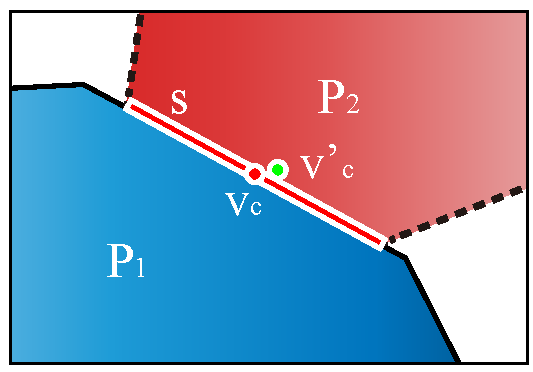
\includegraphics[width=2.5in]{falseclass}
\caption{{\color{red}{Sketch: False classification}}}
\label{fig:falseclass}
\end{figure}

Face classification also suffers from robustness and exactness problems. Many methods classify face according to the indicators of its barycenter, which can be computed by point-in-polyhedron test \cite{feito2013fast,campen2010exact}. However, coordinates of barycenters cannot be exactly represented and have the potential to generate false classification (Fig. \ref{fig:falseclass}). In addition, for the large amount of faces and input meshes, many methods take the benefits of the local coherence of indicators, classifying neighboring faces together \cite{pavic2010hybrid,feito2013fast,ogayar2015deferred,zhou2016mesh}. While this does improve the performance, it can make the robustness problem worse because the false classification may be propagated to neighboring faces.

We want to develop an exact boolean operation method based on the two-step paradigm, being unconditional robust and as fast as possible. Considering the analysis above, we think our method have to include the following features:
\begin{itemize}
    \item Intersection computation has to avoid errors when introducing new vertices into meshes.
    \item All degenerate cases of intersection between input meshes have to be well resolved.
    \item Face classification has to be exact and robust.
    \item Acceleration using geometry connectivity is necessary for face classification.
\end{itemize}

For efficiency, the exactness and robustness should not rely on arbitrary precision arithmetic. Instead, we choose the plane-based techniques from \cite{campen2010exact}. However, as we discussed in section \ref{sec:pbrelated}, BSP structure does not support geometry connectivity query in nature, and we do not want fussy conversions between different representations. Therefore, we use halfedge instead as our major data structure and embed P-rep into it.

\subsection{Intersection-Free Hybrid Mesh}

\begin{figure}[t]
\centering
\includegraphics[width=2.5in]{linkedhalfedge}
\caption{{\color{red}{Sketch: The Linked Halfedge structure}}}
\label{fig:linkedhalfedge}
\end{figure}

\iffalse
\begin{figure*}[!t]
\centering
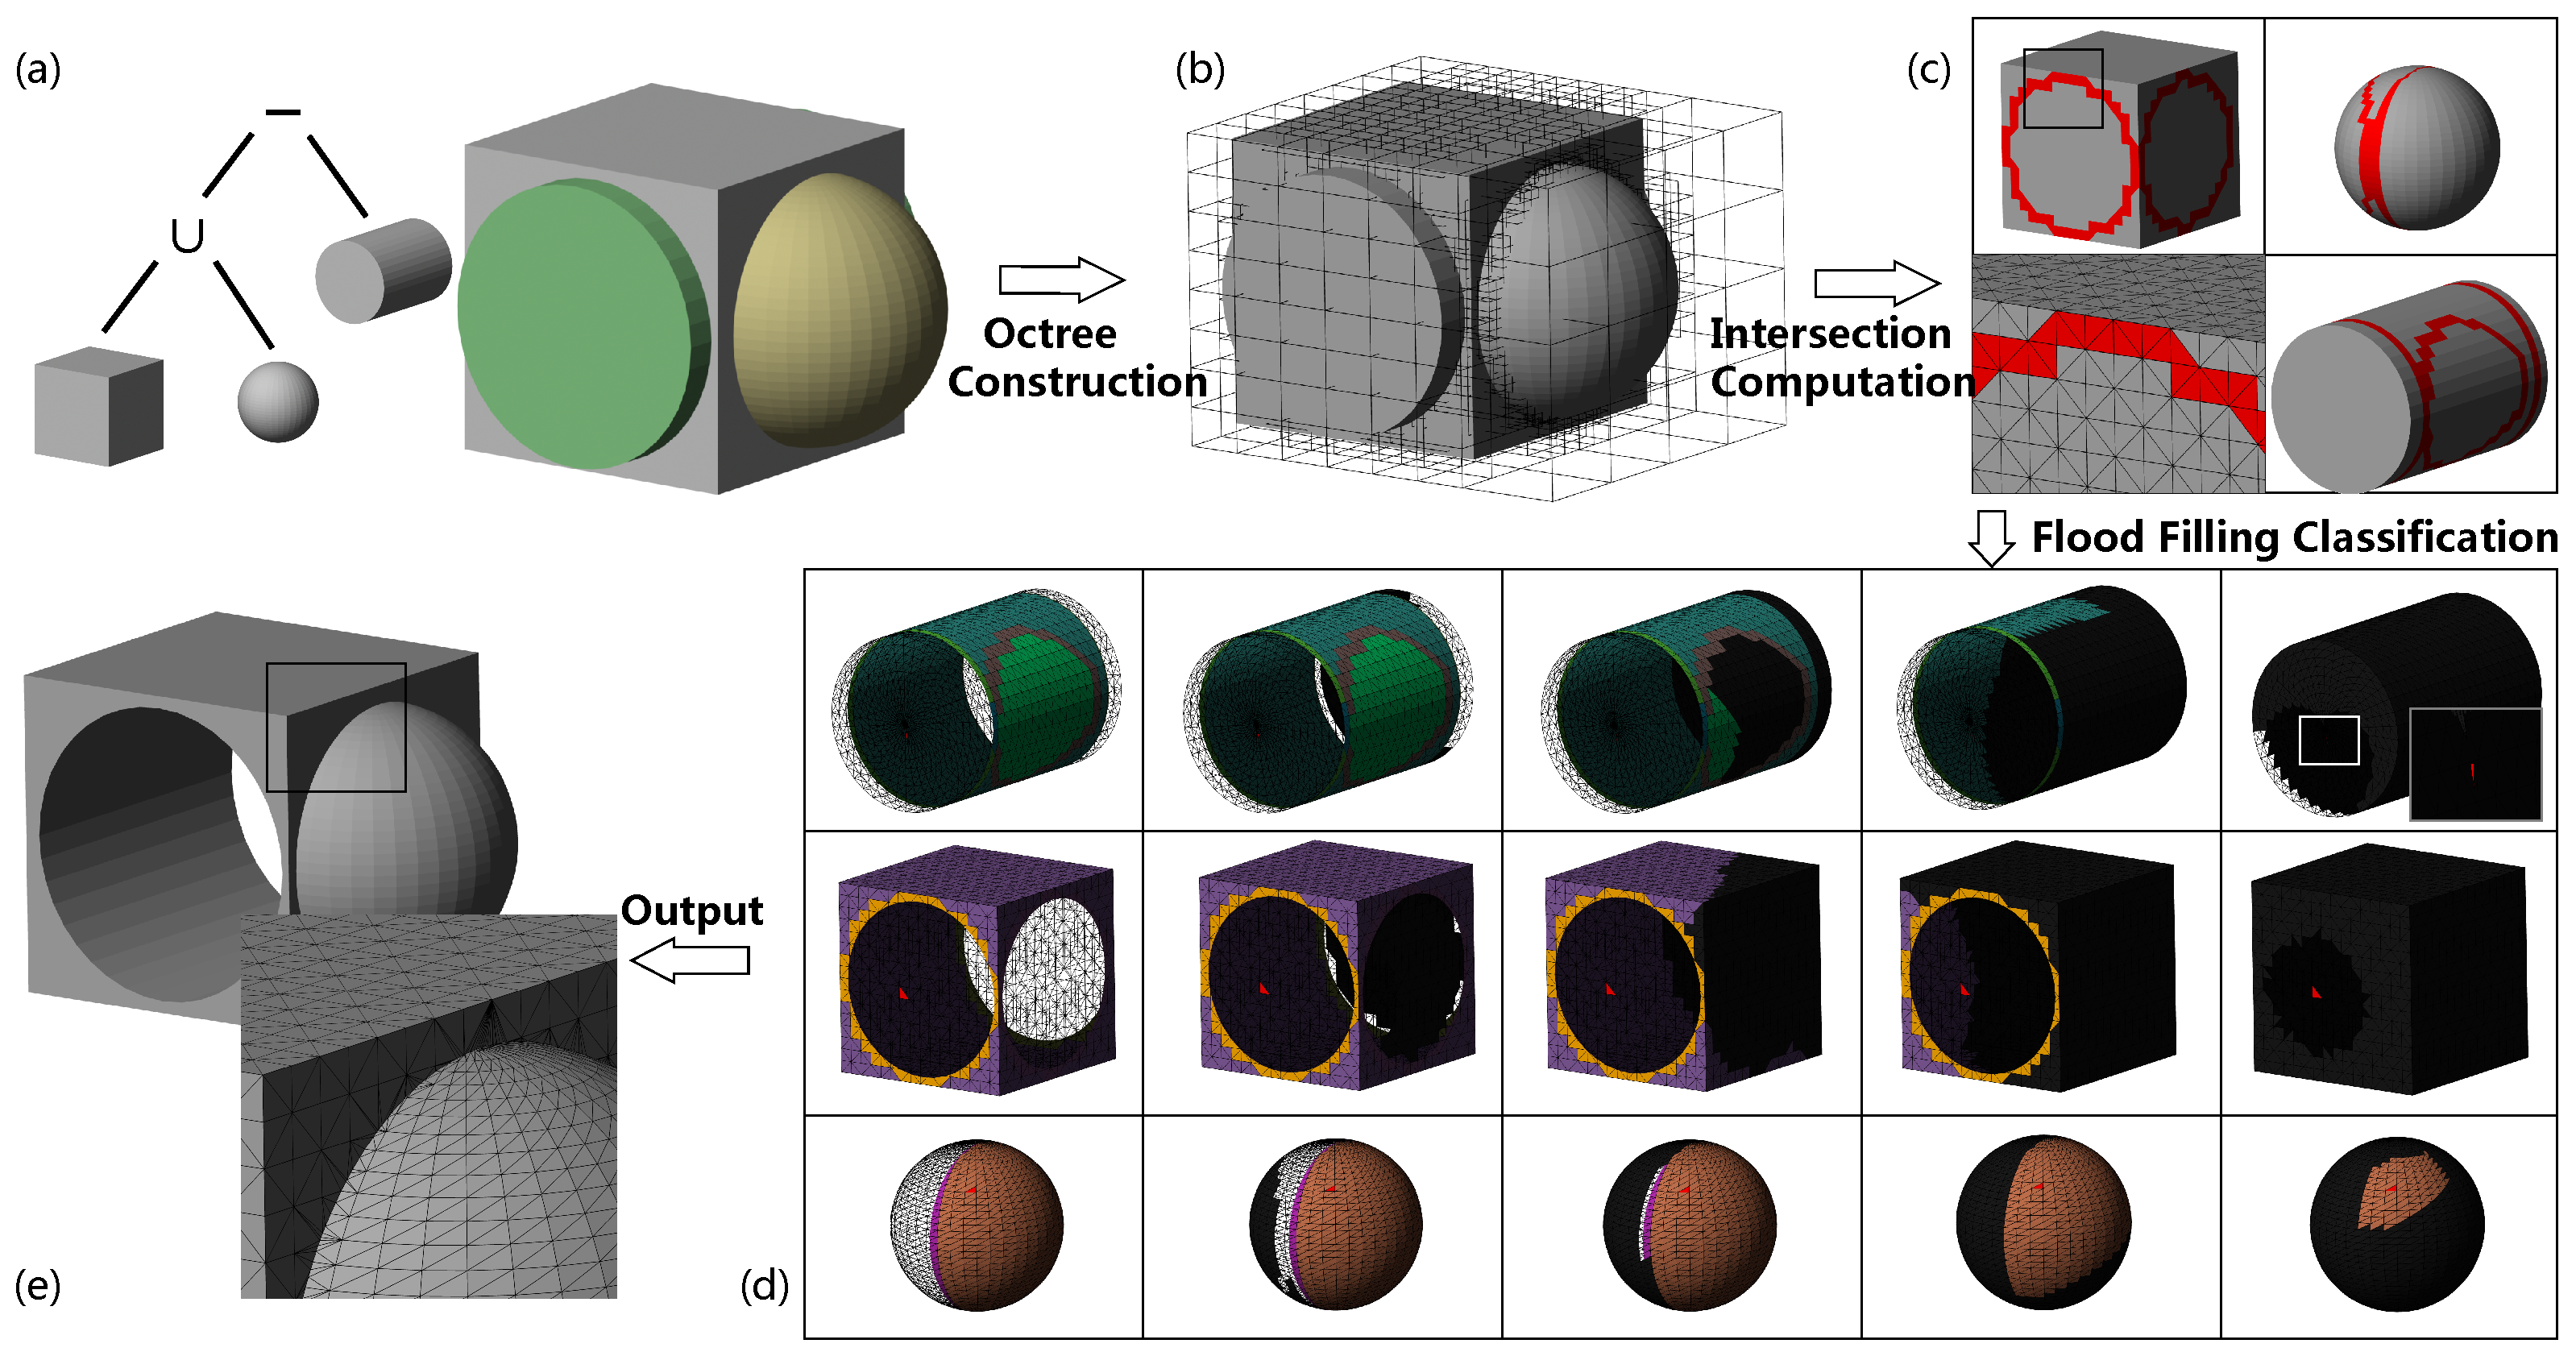
\includegraphics[width=7.1in]{flowchart}
\caption{{\color{red}{Sketch: overview, will be replaced}}}
\label{fig:overview}
\end{figure*}
\fi

\label{sec:meshes}
We made an observation that the non-intersected meshes, as intermediate result of intersection computation, plays an important role of boolean operations. It is a bridge that controls the complexity of intersection computation and facilitates face classification. After the data structure of non-intersected meshes is determined, all things left are how to construct this structure and how to classify according to it.

Our non-intersected mesh, called Linked Halfedge (Fig. \ref{fig:linkedhalfedge}), is a variance of halfedge, a wide-used data structure to represent solids. Halfedge has two advantages: first, since halfedge is popular, using it as the intermediate data structure can avoid unnecessary conversion, which has the potential to have better performance and result topology; second, the geometry connectivity, by which we accelerate classification using local coherence of space indicators, can be easily retrieved through halfedge.

However, naive halfedge is far from enough. The vertex coordinates in halfedge are usually represented by float point number, which cannot exactly represent the newly introduced intersection points. Therefore, we utilize P-rep to avoid computing new coordinates. In addition, we detect all coincident vertices among input meshes (including intersection vertices). This information is used for avoiding repetitive vertices in the final mesh, reconstructing geometry connectivity, and ensuring the topology correctness.

Enlightened by Feito et. al. \cite{feito2013fast}, we found that the the topology near intersection lines between faces can benefit point-in-polyhedron test by dramatically reducing the number of faces needing traversing. Therefore, we add what we call \emph{intersection context} into the our non-intersected meshes to facilitate afterwards face classification. Intersection context identifies where an intersection lies on the surface of the related primitives. An edge of Linked Halfedge stores intersection context only if it is coincident with a certain intersection line segment between primitives. We will give the definition and usage of intersection context in details in section \ref{sec:ir}.

To give an overall impression of Linked Halfedge, we summarize the above content and highlight the features of Linked Halfedge as follows:

\begin{itemize}
  \item Each input mesh is tessellated into a Linked Halfedge by intersection computation.
  \item Coincident vertices between different Linked Halfedge should be linked, that is, coincident vertices are shared among Linked Halfedges.
  \item If a certain edge of Linked Halfedge is coincident with intersection line segment(s), it should be associated with the corresponding intersection context(s).
\end{itemize}


\subsection{Method Overview}


As illustrated in Fig. \ref{fig:overview}, we divide our methods into four steps as follows.

\subsubsection{Space division}

This step is the preparation of intersection detection. As intersection detection is performed between each pair of faces, localization is necessary to filter invalid pairs beforehand. In general, any space division data structure can be applied in this step. We use the adaptive octree for its simplicity. Our implementation is akin to the implementation in \cite{ogayar2015deferred}. Intersection between triangle faces and octree leaves can be efficiently detected using the separating axis theorem \cite{gottschalk1996obbtree}. Octree leaves are classified into two types: if all faces that intersect a leaf belong to the same primitive, we call it a \emph{normal cell}. Otherwise, it is a \emph{critical cell}, within which the following intersection detection is performed.

The difference between our space division and Ogayar et al.'s is that we do not subdivide any normal cell no matter how many faces it contains. This is because subdividing normal cells benefits only the ray-casting point-in-polyhedron test  \cite{frisken2002simple}, which seldom uses in our method. This simplification can save much computing time, especially when intersections between primitives are not complex and located in small regions (e.g. Fig. \ref{fig:models}(x)).

\subsubsection{Intersection detection}

This step is to detect intersections between primitives in a robust and exact way. Our algorithm is largely based on vertex-based M\"{o}ller's algorithm \cite{moller1997fast}, which is very efficient to compute intersection between two triangles. However, naive implementation of M\"{o}ller's algorithm always incurs robustness issues. To avoid an unexpected failure caused by numeric errors, we integrate P-rep of polyhedra into M\"{o}ller's algorithm. All intersection vertices are represented using plane intersections to avoid geometry constructions. Also, we carefully identify all degenerate cases of triangle intersections, including point intersection, line intersection and coplanar intersection, and respectively discuss how to deal with each of them. Details are provided in Section \ref{section:isect}.

\subsubsection{Tessellation}

Once all intersections are detected, we need to tessellate the input primitives and construct the Linked Halfedges. In many methods like \cite{ogayar2015deferred}, constraint Delaunay triangulation (CDT) is applied to perform tessellation, since the intersections are naturally the constraints of CDT. However, for a CSG with more than two primitives, the intersection vertices may be generated by intersections of three faces from different primitives, which cannot be computed during by triangle-triangle intersections in the previous step. Intersection line segments may overlap or intersect with each other, and cannot be used for constraints of CDT directly. In addition, as our intersection vertices are represented exactly by planes, implementation of CDT are complex and inefficient, as most CDT methods were not designed to handle planes and requires explicit coordinates. Therefore, we design a structure suited for P-rep, called \emph{Tess-graph}, to guide the tessellation of each single face, and develop a very fast but exact method to construct Linked Halfedges from Tess-graphs. Details are shown in section \ref{sec:tessellation}.

\subsubsection{Face classification}

This step is to choose faces from the Linked Halfedges to generate the final mesh. Literally computing all the space indicators of each face is unacceptably slow for large CSG trees. We utilize the geometry connectivity to accelerate this process. This is based on the observation that indicators of faces are locally coherent. Many method uses barycenters of faces together with point-in-polyhedra test for face classification, which is not exact nor robust with fix-precision float-point coordinates. Douze et al. \cite{douze2015quickcsg} classifies faces using space indicators of vertices, but failed to deal with coplanar conditions because of coplanar leads to ambiguity in such configurations. Different from all above, we classify faces based on the classification results of exactly represented vertices, including input vertices and newly introduced intersection vertices, and carefully deal with coplanar conditions to ensure topology consistency. Details will be shown in section \ref{sec:classification}.


\section{Plane-based Geometry}

\begin{figure}
  \centering
  % Requires \usepackage{graphicx}
  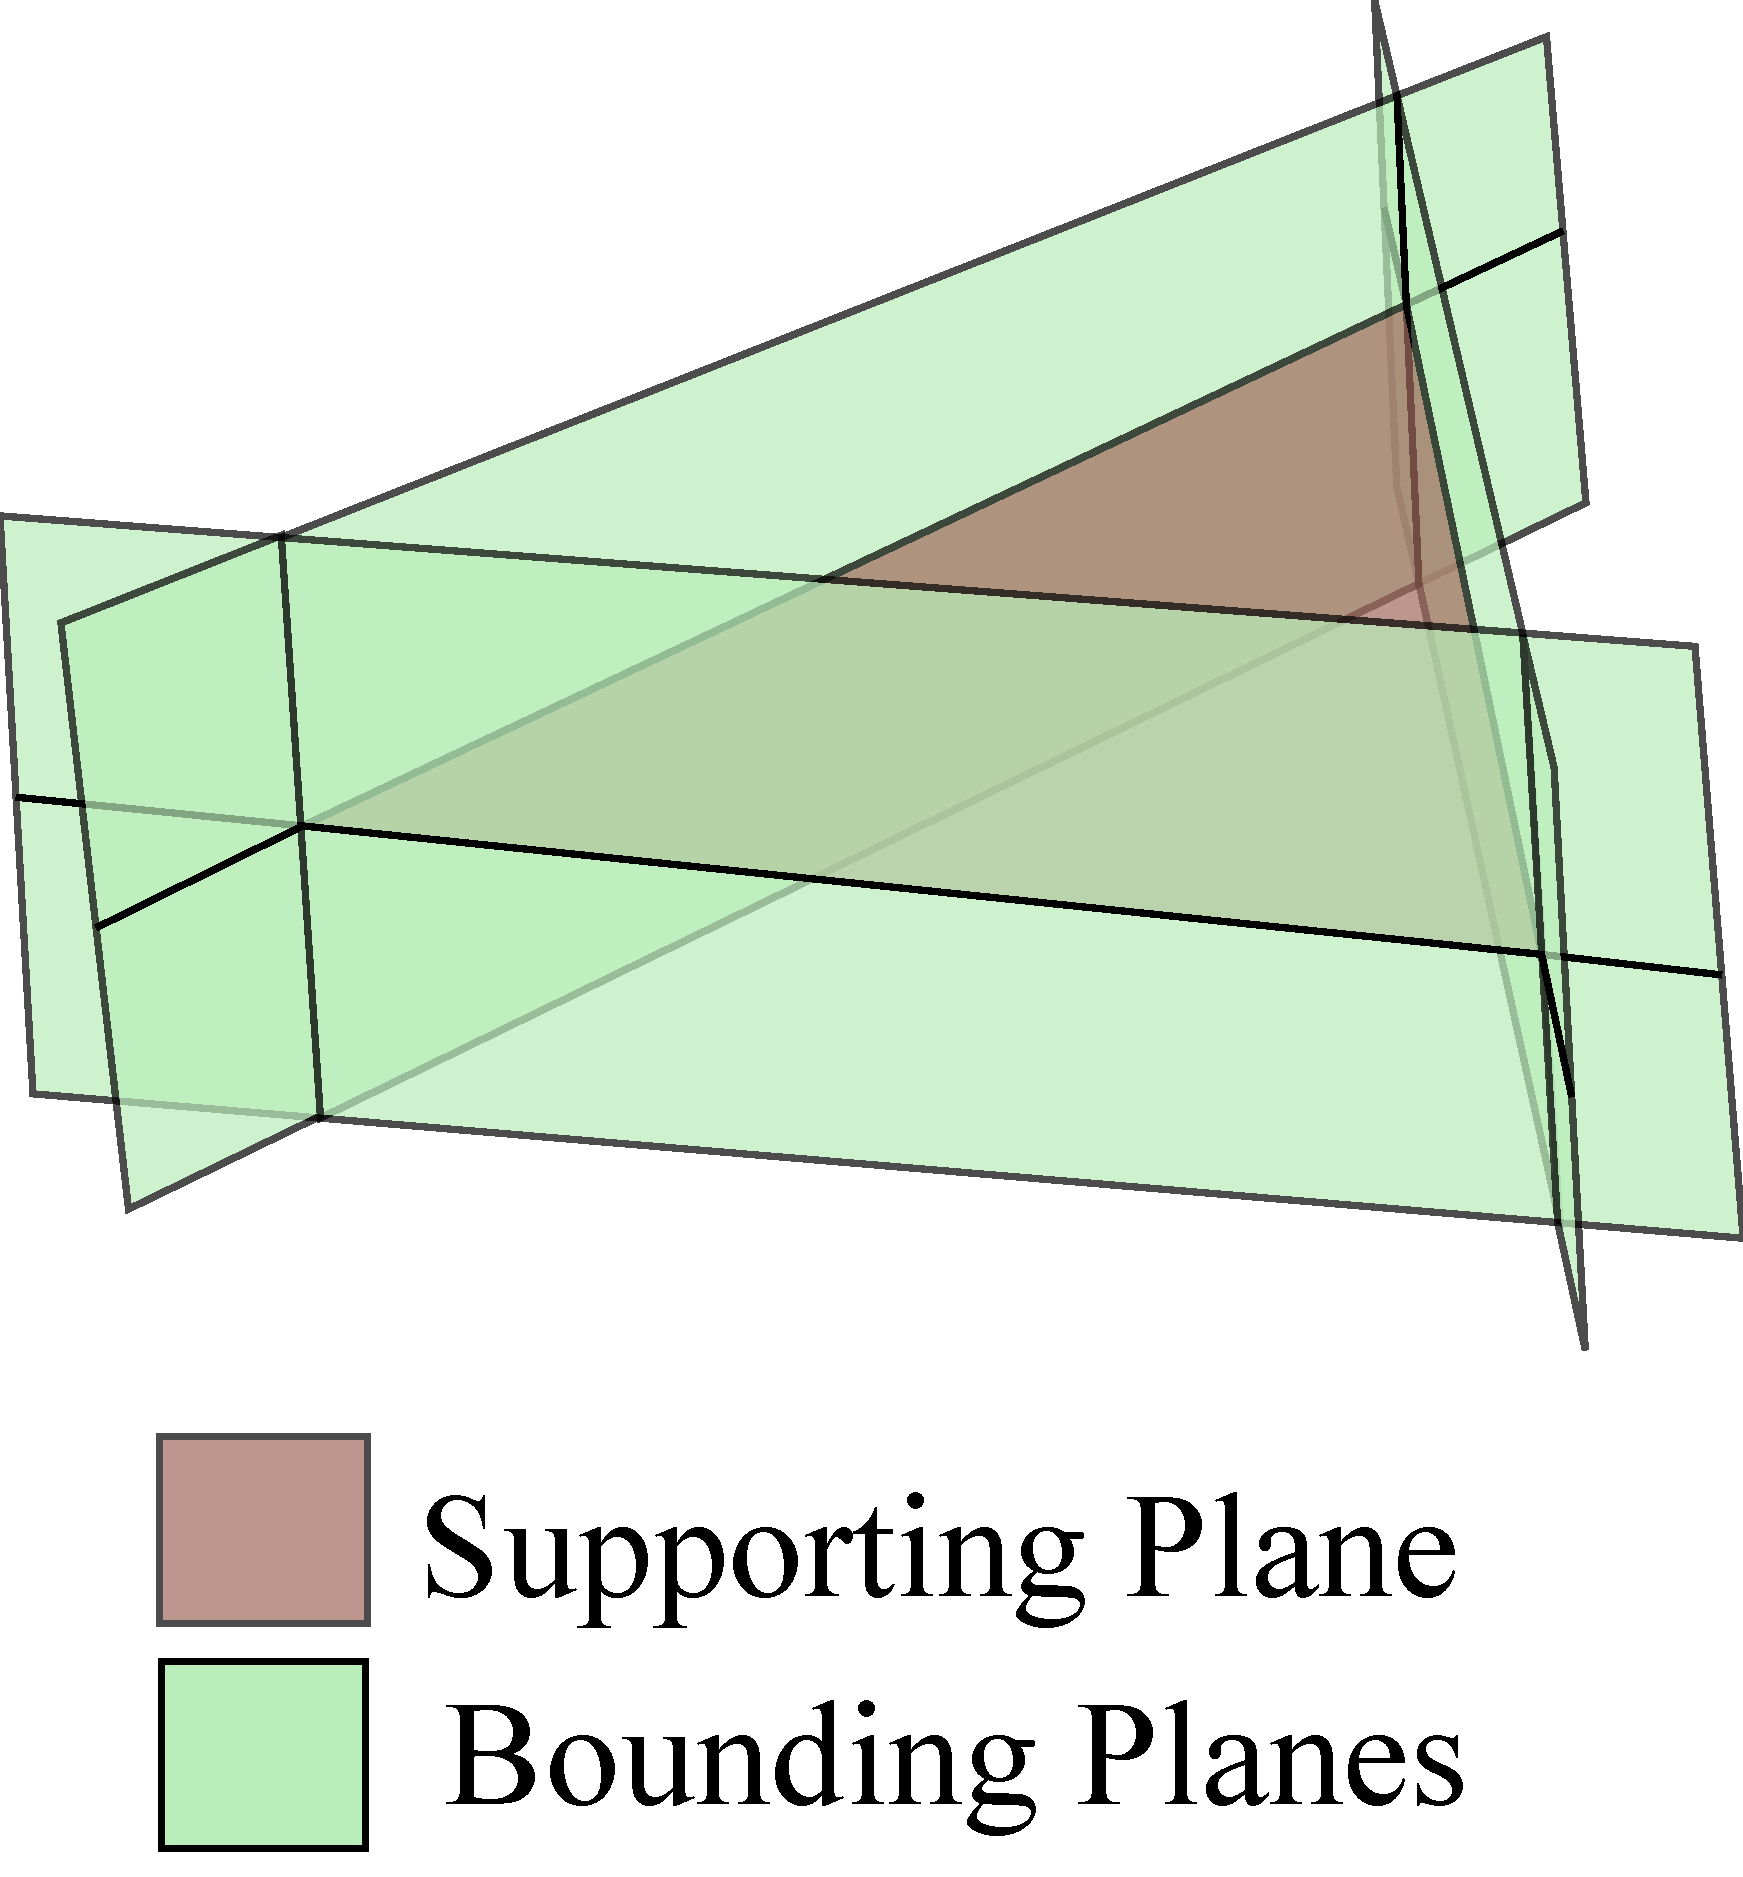
\includegraphics[width=1.7in]{p-reps}\\
  \caption{P-rep of triangles. The yellow triangle is represented by three bounding planes (green) and the supporting plane where the triangle lies.}\label{fig:p-reps}
\end{figure}

As we discussed in Section \ref{sec:paradigm}, one of the problem in boolean operations under vertex-based representation is it inevitably introduces new vertices, whose coordinates cannot be exactly represented using fix-precision float-point number. On the other hand, if P-rep is used, no new geometry information needs to be constructed. Therefore, we can use only geometric decision predicates to perform boolean operations. As the precision of input coordinates is finite, we can determine in advance the upper boundary of precision needed to perform a precise decision, with which we can use fixed precision predicates techniques to gain much performance while keeping exactness. For efficiency, we implement the predicates using filtering techniques proposed by Shewchuk \cite{shewchuk1997adaptive}.

As illustrated in Fig. \ref{fig:p-reps}, using P-rep, each face $f$ with $n$ edges is represented by a supporting plane $\bm{p}_{f,s}$, where the face lies, and a list bounding planes $\{\bm{p}_{f,b}^i \ \vert\  i = 0, 1,...,n-1\}$. Each edge line $\bm{e}_f^i$ is represented by intersection $\bm{p}_{f,s} \cap \bm{p}_{f,b}^i$. Corner vertex $\bm{v}_f^i$ is represented by intersection $\bm{p}_{f,s} \cap \bm{p}_{f,b}^i \cap \bm{p}_{f,b}^{{(i+1)}\bmod{n}}$.

We also introduce some commonly used notations for better presentation in the rest of paper. A plane $\bm{p}$ can be represented by four scalar coefficients $a(\bm{p}), b(\bm{p}), c(\bm{p}), d(\bm{p})$. The normal of $\bm{p}$ is denoted as $\bm{n}(\bm{p})$, which is a normalized vector consisting of the first three plane coefficients. A line $\bm{l}$ can be represented by intersection of two planes $(\bm{p}_l^0 \cap \bm{p}_l^1)$, or in short, $\bm{l}\colon(\bm{p}_l^0 \cap \bm{p}_l^1)$. The positive direction of the line $\bm{l}$ is defined by $\bm{n}(\bm{p}_l^0) \times \bm{n}(\bm{p}_l^1)$. A point $\bm{v}$ can be represented by non-trivial plane triples $(\bm{p}_v^0 \cap \bm{p}_v^1 \cap \bm{p}_v^2)$, or in short, $\bm{v}\colon(\bm{p}_v^0 \cap \bm{p}_v^1 \cap \bm{p}_v^2)$.


\subsection{Conversion}

\label{sec:convert}

We use Campen et al.'s method \cite{campen2010exact} for exact conversion of triangles (represented by three vertices) from vertex-based representation to P-rep. Given that the input vertex coordinate has $L$-bit precision including sign, the precisions of the four plane coefficients are $L_a, L_b, L_c, L_d$, which have to meet the following requirements:
\begin{equation}
\begin{split}
&L_a=L_b=L_c\ge 2(K-1)+1+1,\\
&L_d\ge(L_a-1)+(L-1)+2+1.
\end{split}
\end{equation}
Here $K$ is the maximum bits required to represent edge vector components in input meshes. If we use $M$ bits to store each plane coefficient, basically $M$ has to be greater than $L_d$. In our implementation, we actually use a more strong constraint $M \ge L_d+1$. Under this constraint, given a $L$-bit vertex $\bm{v_i}$, we can compute the orientation of plane $p_j$ with respect to $\bm{v_i}$ by the sign $\bm{n}(\bm{p_j})\cdot\bm{v_i} + d(\bm{p_j})$, which can be exactly computed using common float point arithmetic with limited $M$-bit precision. It allows very fast plane orientation predicates which benefits much the early rejection in our intersection computation (\S \ref{section:isect}).


Let $\delta = 2^{K-L-1}$ be the relative length (in max-norm) of the longest edge in the mesh (relative to the bounding box). If we use IEEE 754 double float point number ($M=53$) and assume $\delta \le 2^{-5.5} \approx 0.022$, the maximum input precision $L$ can reach to 20, which is enough for most application (for standard IEEE 754 single float point number, the precision is 24-bit).


\subsection{Substrates}
\label{sec:substrates}
Plane-based geometry predicates include checking coincidence and co-orientation of planes, orientation of a plane with respect to a point, and whether three planes intersect in a unique point, etc. Most of them are well-discussed in previous work \cite{bernstein2009fast,banerjee1996topologically}. In the following, we focus on two advanced plane-based predicates---\emph{point ordering on line} and \emph{circular ordering of line}, which are important building blocks of our method.

\vspace{0.5em}
\noindent \textbf{Linear ordering on points}~~~~
Given an arbitrary line $\bm{l}$ with two points $\bm{v}_1\colon(\bm{p}_1^0\cap\bm{p}_1^1\cap\bm{p}_1^2)$ and $\bm{v}_2\colon(\bm{p}_2^0\cap\bm{p}_2^1\cap\bm{p}_2^2)$ on it, we need to determine the linear order of the two points along $\bm{l}$ (Fig. \ref{fig:twopointoneline}). To solve this problem, we choose one plane not parallel with $\bm{l}$ from the plane representation of each point. Then we convert this problem into linear order of planes and solve it using the same technique as Banerjee et al. \cite{banerjee1996topologically}. The chosen planes should have the same orientation with $\bm{l}$ (the dot product between plane normal and $\bm{l}$ has to be positive) and unqualified planes have to be flipped.


\vspace{0.5em}
\noindent \textbf{Circular ordering of lines}~~~~
During face tessellation, we need to know the which edges are neighboring (Fig. \ref{fig:circularorder}), that is, circular ordering of directed lines around a vertex. Lines can be sorted in a divide-and-conquer way based on the relative order of each pair of lines. Therefore, this problem is converted to that given two coplanar lines $\bm{l}_a\colon(\bm{p}_a^0\cap\bm{p}_a^1)$ and $\bm{l}_b\colon(\bm{p}_b^0\cap\bm{p}_b^1)$ with their intersection point $\bm{v}_{ab}$, compute the circular order of the two lines. Supposing the common plane is $\bm{p}_s$, we can compute the order by the sign of $\sin{\theta_{ab}}$, where $\theta_{ab}\in(-\pi,\pi)$ is the angle from $\bm{l}_a$ to $\bm{l}_b$ under the top view of $\bm{p}_s$. And the sign of sine is the same as triple product $\bm{n}(\bm{p}_s) \cdot (\bm{l}_a\times\bm{l}_b)$,
where $\bm{n}$ means the normal direction. However, explicit computing this equation is complicated because both $\bm{l}_a$ and $\bm{l}_b$ are implicitly represented by intersection of planes.

We develop an easier way that requiring no explicit computation of $\bm{l}_a$ and $\bm{l}_b$. We orthogonally decompose $\bm{n}(\bm{p}_a)$ and $\bm{n}(\bm{p}_b)$ along the normal the common plane $\bm{p}_s$:
\begin{equation}
\begin{split}
&\bm{n}(\bm{p}_a)= \bm{n}^\parallel(\bm{p}_a) + \bm{n}^\perp(\bm{p}_a)\\
&\bm{n}(\bm{p}_b)= \bm{n}^\parallel(\bm{p}_b) + \bm{n}^\perp(\bm{p}_b)
\end{split}
\end{equation}
Here superscript `$\parallel$` means the projection on $\bm{p}_s$ and `$\perp$` means orthogonal to $\bm{p}_s$. As we know $\bm{n}^\perp(\bm{p}_a)$ and $\bm{n}^\perp(\bm{p}_b)$ are both parallel to $\bm{n}(\bm{p}_s)$, we get:
\begin{equation}
\label{eq:circ1}
\bm{n}(\bm{p}_s) \cdot (\bm{n}(\bm{p}_a) \times \bm{n}(\bm{p}_b)) = \bm{n}(\bm{p}_s) \cdot (\bm{n}^\parallel(\bm{p}_a) \times \bm{n}^\parallel(\bm{p}_b)).
\end{equation}
By simple geometry reasoning, we find that the angle between $\bm{n}^\parallel(\bm{p}_a)$ and $\bm{n}^\parallel(\bm{p}_b)$ is exactly $\theta_{ab}$. So the sign of the right side of equation \ref{eq:circ1} is exactly the sign of $\sin{\theta_{ab}}$. It means we have the following nice conclusion:
\begin{equation}
\label{eq:circ2}
sign(\sin{\theta_{ab}})=  sign(\bm{n}(\bm{p}_s)\cdot(\bm{n}(\bm{p}_a) \times \bm{n}(\bm{p}_b)))
\end{equation}

Since all the three vectors are already explicitly represented, we only have to evaluate the sign of an 3x3 matrix and avoid complicated high precision float-point arithmetic.
\begin{figure}
  \centering
  % Requires \usepackage{graphicx}
  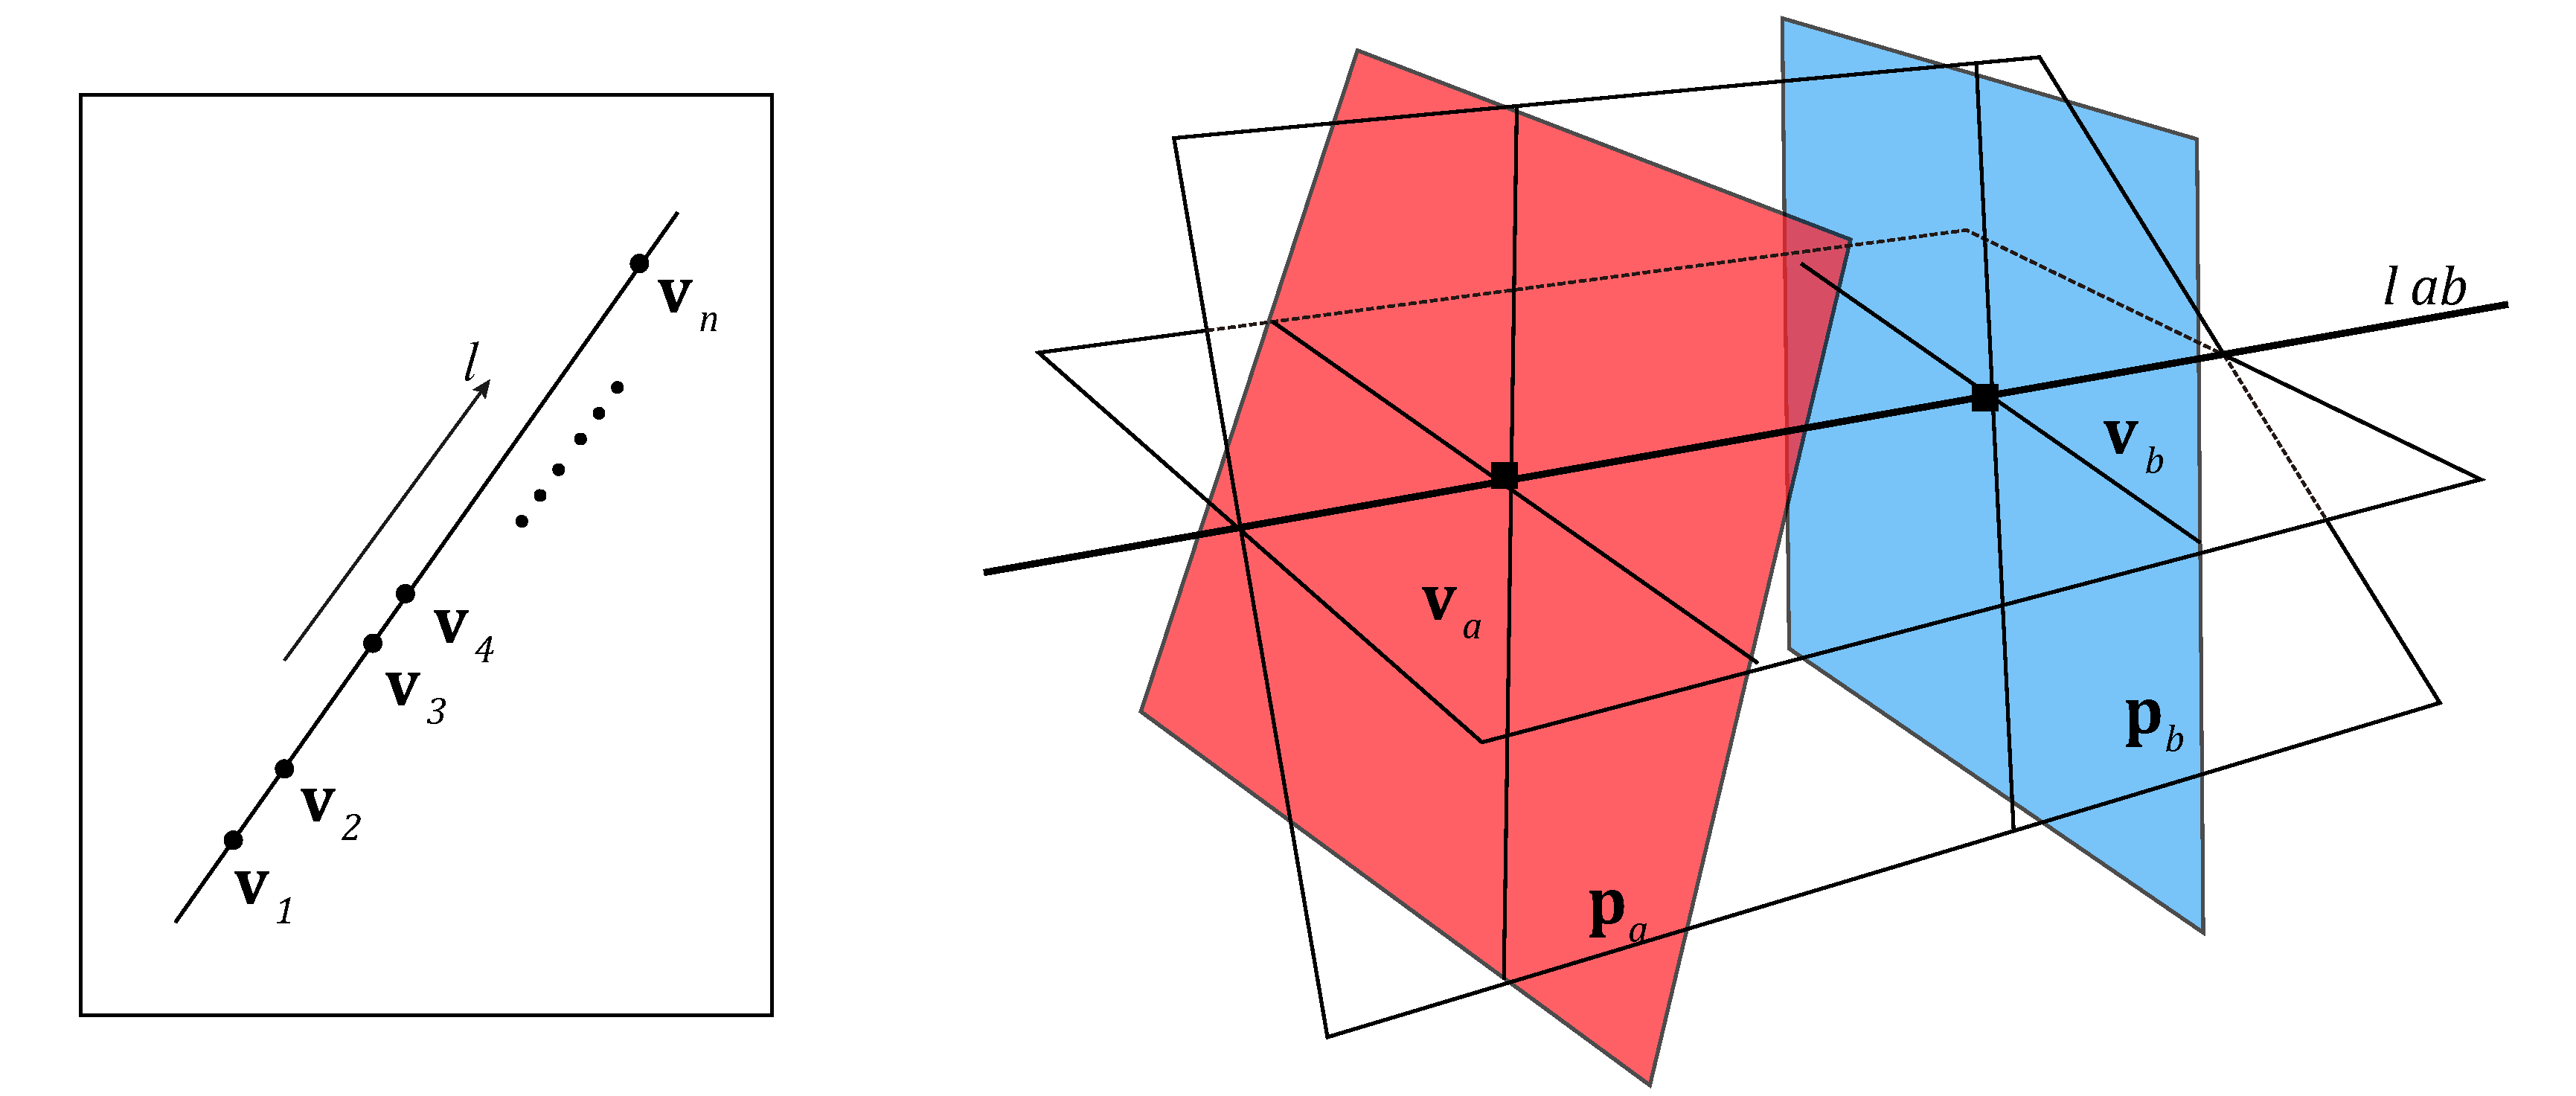
\includegraphics[width=2.5in]{twopointoneline}\\
  \caption{{\color{red}{Sketch: config of two point one line comparison}}}\label{fig:twopointoneline}
\end{figure}

\begin{figure}[t]
\centering
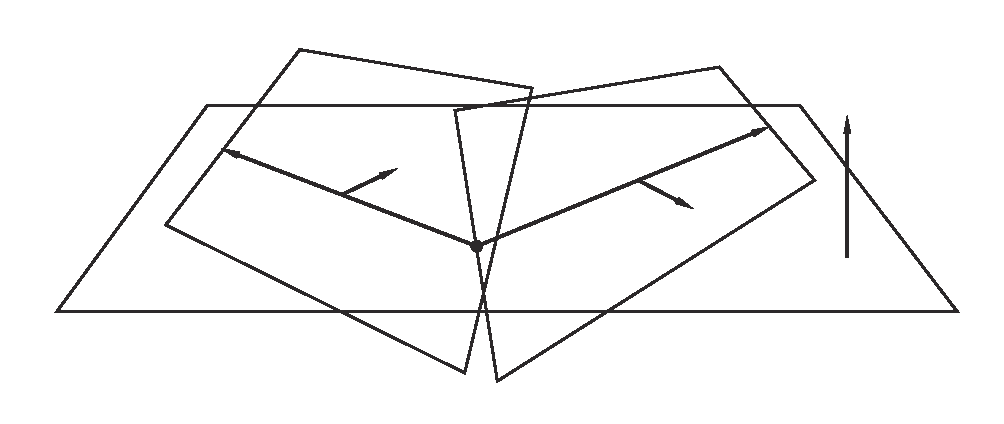
\includegraphics[width=2.5in]{circularorder}
\caption{The configuration of two-line-one-plane comparison. $l_a\colon(p_0, p_a)$ and $l_b\colon(p_0, p_b)$ are coplanar in $p_0$. We want to compute $sign(\vec{n}_0 \cdot (\vec{l}_a \times \vec{l}_b))$.}
\label{fig:circularorder}
\end{figure}


\section{Exact Intersection Computation}

\label{section:isect}
In this step, intersections between faces are computed through triangle-triangle intersection test. We adopt M\"{o}ller's algorithm \cite{moller1997fast} on account of its efficiency and simplicity. However, a naive implementation of M\"{o}ller's algorithm may fail to produce correct results because of numerical errors. Therefore, we integrate plane-based geometry representation to make it unconditionally exact and robust. In the following, we first make a quick review of M\"{o}ller's algorithm, and then discuss the way to integrate plane-based geometry. After that, we talk about how to deal with degenerate cases.

\subsection{M\"{o}ller's Vertex-Based Method}

\begin{figure}[t]
\centering
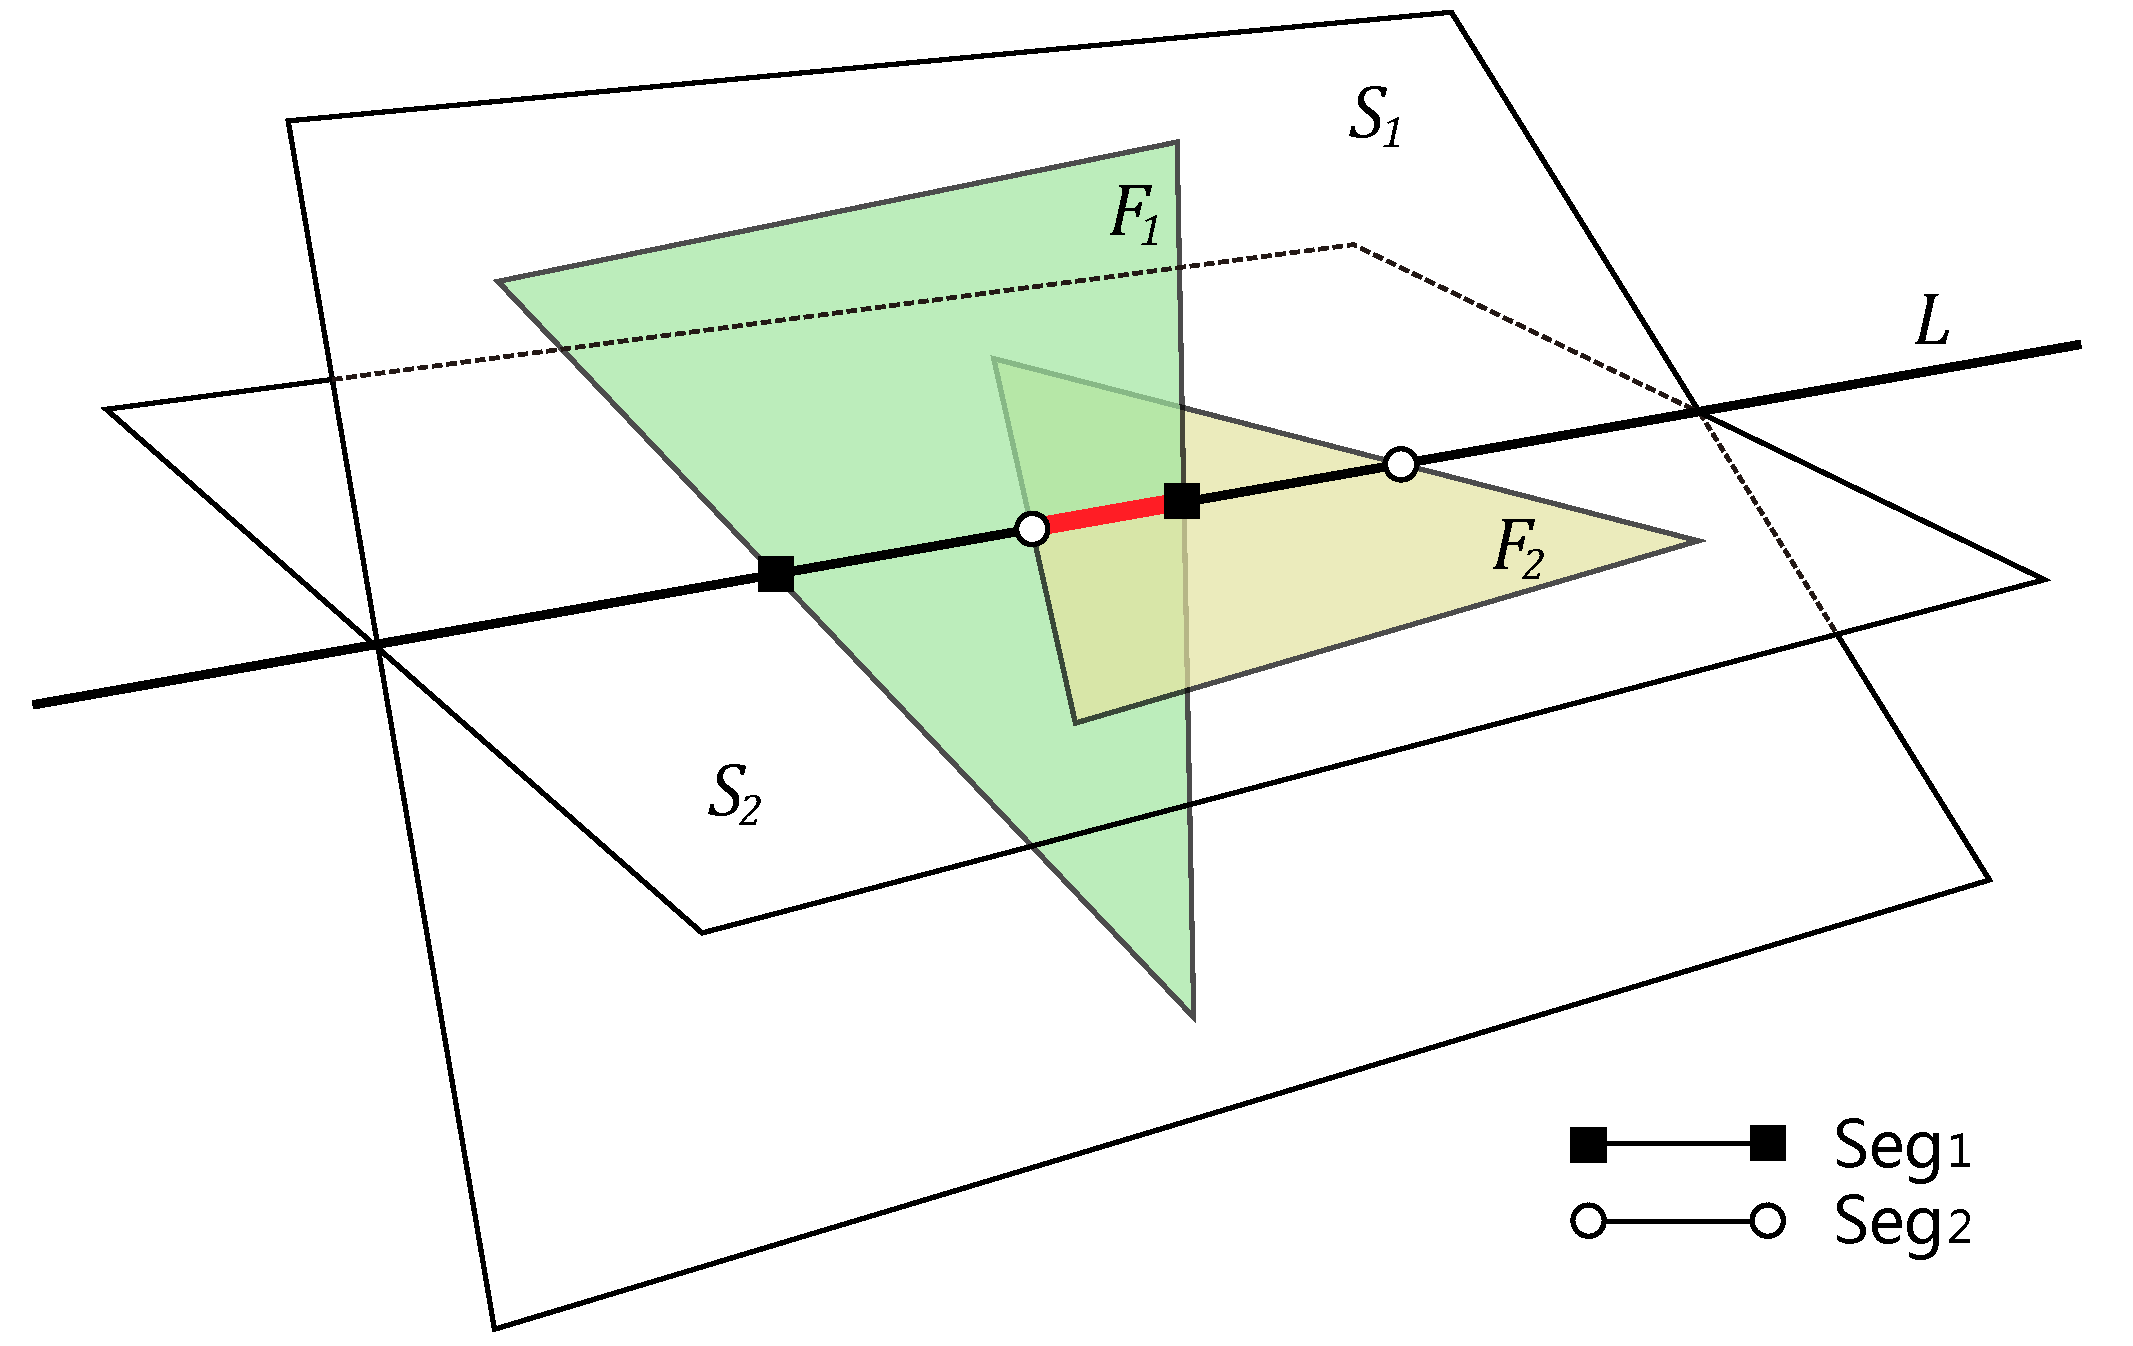
\includegraphics[width=2.5in]{projection}
\caption{$Seg_1$ is the intersection between $p^s(t_2)$ and $t_1$. $Seg_2$ is the intersection between $p^s(t_1)$ and $t_2$. The intersection between $t_1$ and $t_2$, which is the line segment in red, is the overlap of $Seg_1$ and $Seg_2$.}
\label{fig_projection}
\end{figure}


M\"{o}ller's algorithm computes the intersection between two triangles $t_1$ and $t_2$ in three steps as shown in Fig. \ref{fig_projection}:
\begin{itemize}[leftmargin=0.45cm]
\item[1)] An early rejection is performed by testing whether $t_1$ intersects $\bm{p}_{t_2, s}$, the supporting plane of $t_2$. The same test is also done between $t_2$ and $\bm{p}_{t_1, s}$.
\item[2)]The intersection between $t_1$ and $\bm{p}_{t_2, s}$, denoted as $Seg_1$, and the intersection between $t_2$ and $\bm{p}_{t_1, s}$, denoted as $Seg_2$, are separately computed .
 \item[3)]The intersection between $t_1$ and $t_2$ is determined by computing the overlap between $Seg_1$ and $Seg_2$ .
\end{itemize}

The non-robustness of this algorithm is from computing the coordinates of intersection vertices, which is the end points of $Seg1$ and $Seg2$. Although implementation with arbitrary precision arithmetic produces exact coordinates, it is too costly for boolean operations of large CSG. We use plane-based geometry to solve this problem by implicitly representing intersections with planes.


\subsection{Plane-based Technique Embedding}

\label{sec:embed}
According to the method described in section \ref{sec:convert}, triangle faces $f$ are firstly converted to its P-rep: a supporting plane $\bm{p}_{t, s}$ surrounded by three bounding planes $\{\bm{p}_{t, b}^i|\ i = 0,1,2\}$. We integrate the plane-based geometry into each of the tree steps of M\"{o}ller's algorithm as following:

\begin{figure}[t]
\centering
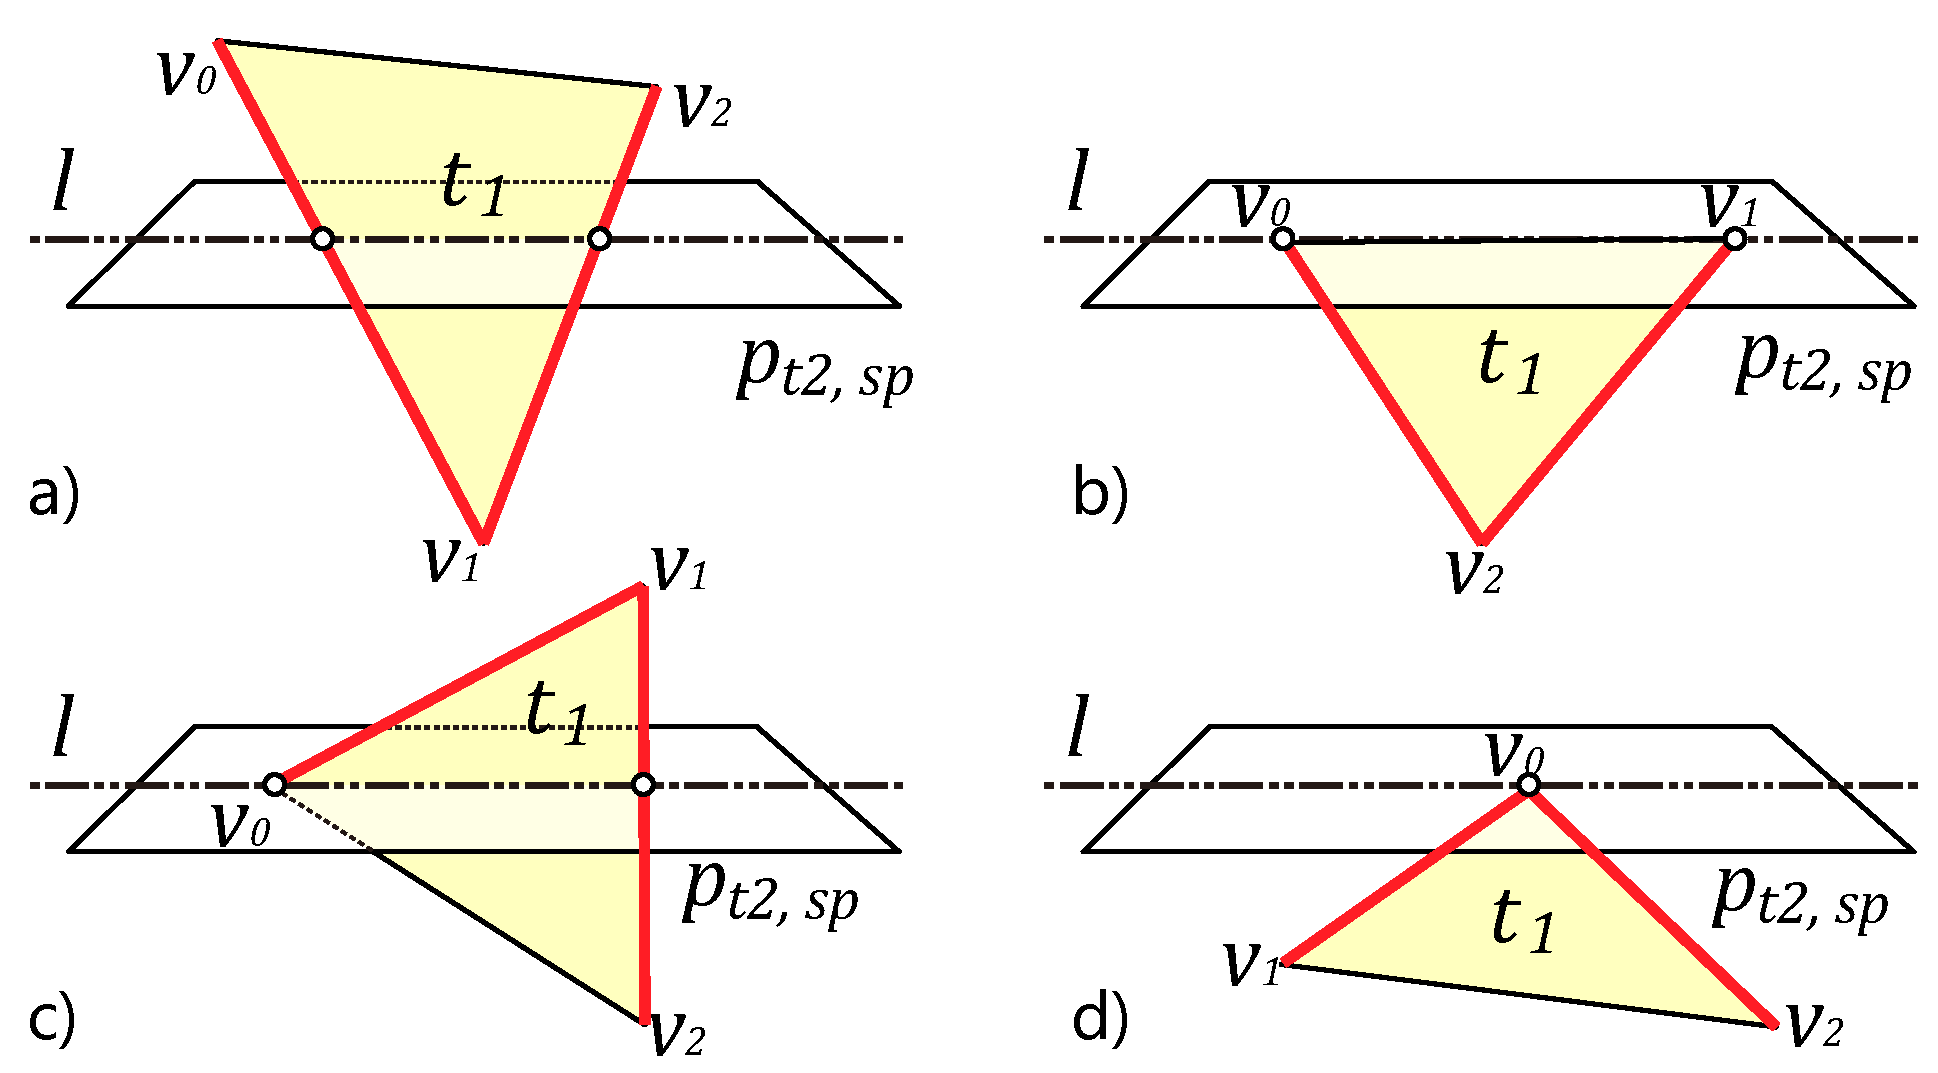
\includegraphics[width=3.5in]{sign}
\caption{We denote the signed distance from point $X$ to plane $S_2$ as $d_X$. All the four conditions of intersection between $t_1$ and $S_2$ (denoted as $Seg_1$) are:  (a) $d_A\cdot d_C<0$, $d_B\cdot d_C<0$; (b) $d_A=0$, $d_B=0$, $d_C\neq 0$; (c) $d_A=0$, $d_B\cdot d_C<0$; (d) $d_A=0$, $d_B\cdot d_C>0$. End points of $Seg_1$ are intersections between $S_2$ and related edge lines of $t_1$ (bold edges).}
\label{fig:isect}
\end{figure}



\begin{itemize}[leftmargin=0.45cm]
  \item[1)] The basic subroutine of the first step is given two faces $t_1$ and $t_2$, computing the orientation of of a face with respect to vertices from the other face. Reviewing the discussion of \S \ref{sec:convert}, under the constraint of $M \ge P+1$, we can compute the predicate within the precision of $M$ bits. This allow us to perform this early rejection efficiently.
      \vspace{0.5em}
  \item[2)] If $t_1$ and $t_2$ are not coplanar, the end points of $Seg_1$ and $Seg_2$ can be implicitly represented by plane triples. Take $Seg_1$ as an example. $Seg_1$ is the intersection between $t_1$ and $\bm{p}_{t_2, s}$ and the end points of $Seg_1$ are intersections between $\bm{p}_{t_2, s}$ and edges from $t_1$ (denoted as $\bm{e}^i_{t_1}$). Because $\bm{e}^i_{t_1}$ can be represented as $\bm{p}_{t_1, s}\cap \bm{p}^i_{t_1, b}$, the end points of $Seg_1$ can be represented in the form of $\bm{p}_{t_2, s} \cap \bm{p}_{t_1, s} \cap \bm{p}^i_{t_1, b}$. In Fig. \ref{fig:isect}, we list all possible intersecting situations between $t_1$ and $\bm{p}_{t_2, s}$. The two corresponding bounding planes $\bm{p}^i_{t_1, b}$ for each situation are also presented. The coplanar condition will be discussed later in \S \ref{sec:degenerate}.
      \vspace{0.5em}
 \item[3)] The intersection between $t_1$ and $t_2$ is the overlap area of $Seg_1$ and $Seg_2$. It can be easily computed by sorting the end points of $Seg_1$ and $Seg_2$ along the line $\bm{l}\colon \bm{p}_{t_1, s} \cap \bm{p}_{t_2, s}$. Because end points are all represented using plane triples, we can use the linear order of points discussed in \S \ref{sec:substrates} to sort.
\end{itemize}

Each time an intersection is computed, two intersections are generated (one for each triangle) and the newly generated vertices are added into meshes. To avoid repetitive vertices in the final result, we perform vertex repetition elimination in this stage, merging coincident vertices even among different input meshes. Because we use P-reps, the comparison of vertices is exact.

\subsection{Plane-Based Intersection Representation}
\label{sec:ir}

Once intersections are computed, proper representation is needed to guarantee exact transfer of information and low cost to process. In our method, an intersection line segment $\mathbb{I}$ is represented by our plane-based intersection representation (PBI-rep) as $\{t, \bm{p}_{ext}, (\bm{p}^0, \bm{p}^1),\bm{\Psi}\}$. The first component indicates $\mathbb{I}$ is on triangle $t$, and second one $\bm{p}_{ext}$ indicates $\mathbb{I}$ lies on a line $\bm{l}_{\mathbb{I}}\colon(\bm{p}_{t, s} \cap \bm{p}_{ext})$. The two end points of $\mathbb{I}$ are $\bm{l}_{\mathbb{I}}\cap\bm{p}^0$ and $\bm{l}_{\mathbb{I}}\cap\bm{p}^1$. The last component $\bm{\Psi}$ is a vector that represents the neighborhood of the intersection, which is for fast face classification in later stages. For each component of $\bm{\Psi}$, if $\mathbb{I}$ is on the surface of primitive $P_k$, the $k^{th}$ component $\Psi_{k}$ is the edge or face of $P_k$ where $\mathbb{I}$ lies. Otherwise, $\Psi_{k}=0$, meaning default empty data.

To illustrate, assume two triangle faces $t_1$ and $t_2$, from primitive $P_a$ and $P_b$, intersect on a line segment. Then it generates two intersections for both triangles respectively, denoted as ${\mathbb{I}}_{12}$ and ${\mathbb{I}}_{21}$. For ${\mathbb{I}}_{12}$, the first two components are $t_1$ and $\bm{p}_{t_2, s}$. The computation of the third component is discussed in \S\ref{sec:embed}. The neighborhood $\bm{\Psi}$ is zero for all components except $\Psi_a$ and $\Psi_b$. In most time, $\Psi_a=t_1$ and $\Psi_b=t_2$. However, sometimes, intersections may lie on the primitive edges instead of faces. In that case, $\Psi_a$ and $\Psi_b$ are edges. We postpone this discussion until \S\ref{sec:degenerate}. The computation of ${\mathbb{I}}_{21}$ is similar.


\subsection{Degenerate Case Handling}
\label{sec:degenerate}

Which two triangles, if intersecting, intersect on a line segment in most situations, they can also intersect on a point or a convex area (coplanar case). Even if line segment is the intersection, the intersection can be on triangle edges or inside triangles. These degenerate situations are troublesome to develop a robust boolean method. In this section, we offer simple but robust way to deal with all the degenerations and conceal the complexity of intersections behind the concise intersection representation in \S\ref{sec:ir}.


%The criterion of whether an intersection help tessellation is by its necessity: if the intersection is not presented, whether some faces from the linked halfedge will cross the boundary of primitives. The word 'cross' do not only include the situation that a face is partly outside and partly inside of a primitive, but also can mean that a face is partly inside (outside) and part on the boundary of the primitive.

\subsubsection{Point intersection}
\label{sec:ipoint}
If two triangles intersect on a single point (Fig. \ref{fig:isolated}), the intersection cannot be represented using our four-component description. Therefore, we simply add the intersection point into the meshes to guarantee correct tessellation, and no intersection is introduced.

\begin{figure}[t]
\centering
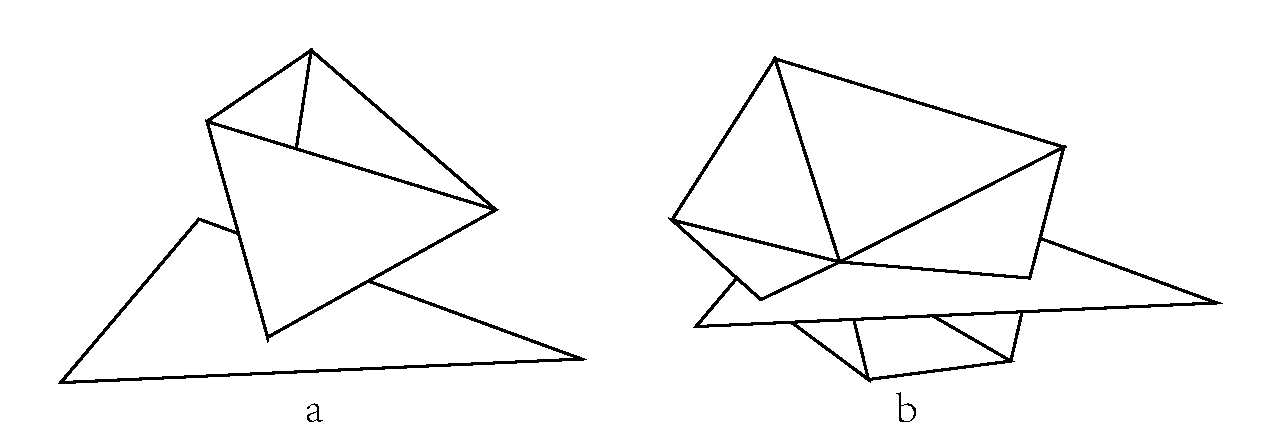
\includegraphics[width=3.5in]{isolated}
\caption{Two situations of point intersections. (a) The intersection point is isolated, and there is no adjacent intersection line segment. This situation may cause non-manifold surface in Boolean operation. (b) The intersection point is not isolated. The intersection point can be introduced by other face pairs during intersection tests.}
\label{fig:isolated}
\end{figure}


\subsubsection{Edge intersection}

% intersect on face edges does not create new line segments, it is part of the edges from other meshes, and will to be duplicated.


% whose edge? need to be further explained and better defined. an edge intersection divide edge in a triangle and will be duplicated in the other


When intersection line segment lies on an edge (Fig. \ref{fig:twin}). we call it \emph{edge intersection}. The only difference between edge intersection and the general case is the neighborhood representation $\Psi$. The space near edge intersection is decided by both face in the two side of the intersected edge, instead of just one triangle face (Fig. X). Therefore, supposing intersection is on the edge from mesh $P_k$, the neighborhood $\Psi_k$ is then an edge. Note that an intersection can be on edges from different meshes. Then there are more than one component of $\bm{\Psi}$ are edges.

One thing need to be noticed is that there will be repetitive detection of edge intersections. In Fig. \ref{fig:twin}a, the same intersection on $t_1$ will be detected twice with both $t_2$ and $t_2^{\star}$. We solve this duplication together with other interactions among intersections in \S\ref{sec:tessellation}. We call such $t_2$ and $t_2^{\star}$ as \emph{companion triangles} in an edge intersection, a concept which will be referred again in the discussion of coplanar cases.

\begin{figure}[t]
\centering
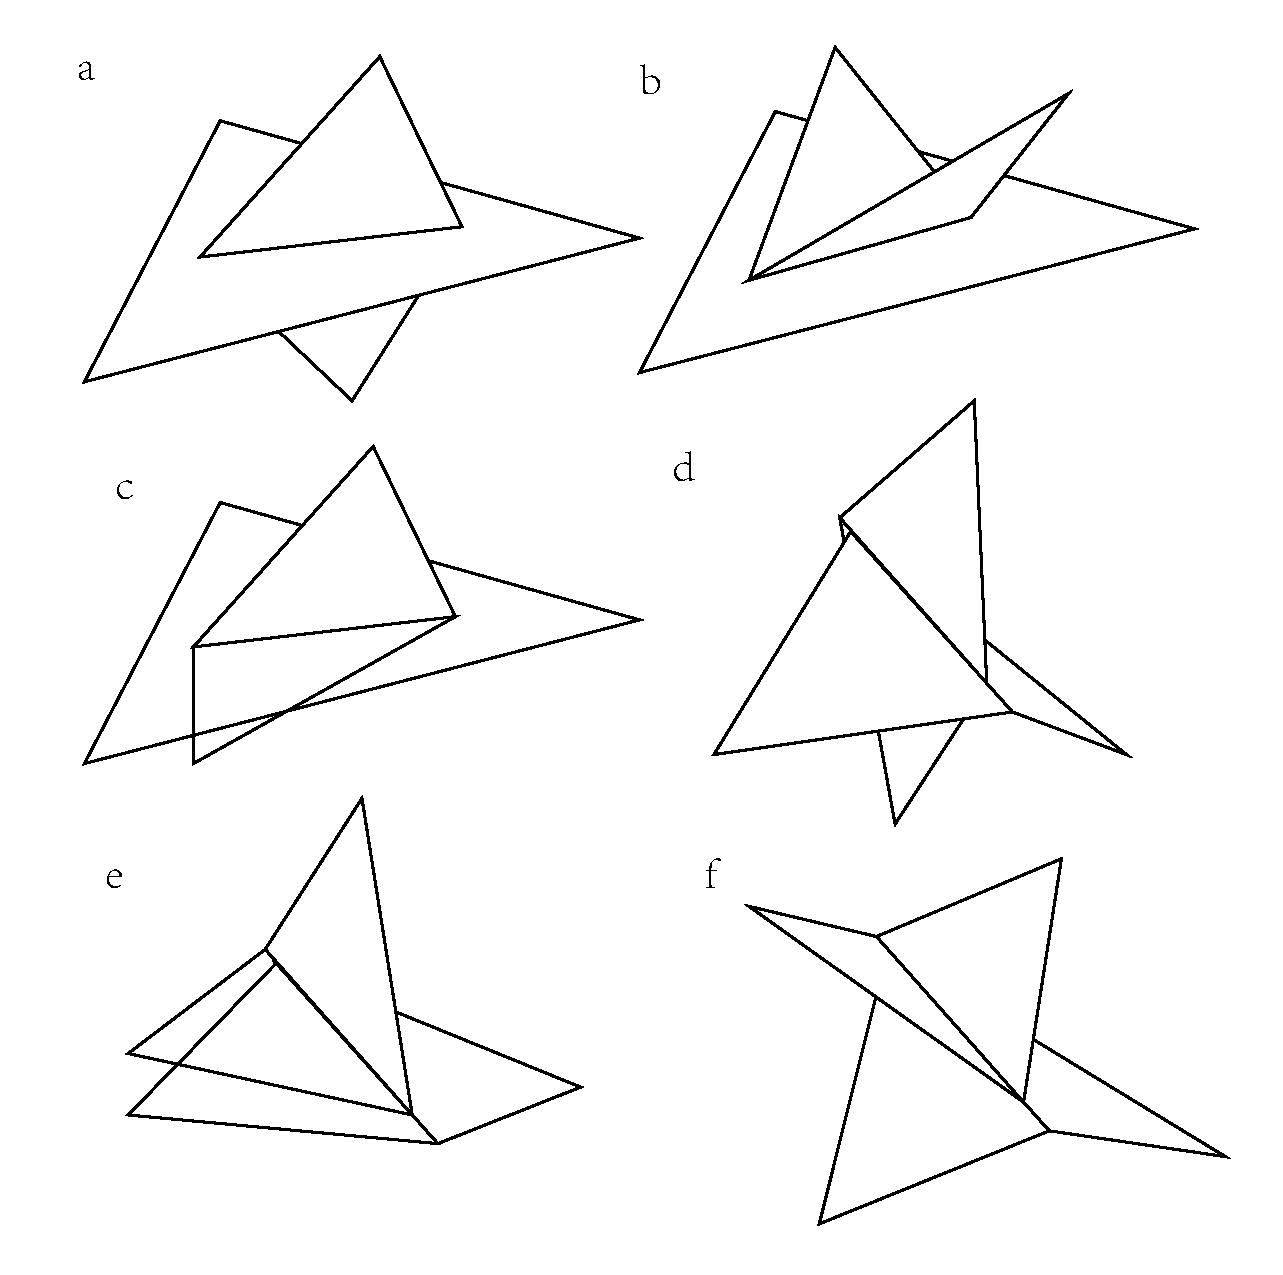
\includegraphics[width=3.5in]{twin}
\caption{Six situations of edge intersections. The first three subgraphs are edge-face intersections. The last three ones are edge-edge intersections. (a) Triangles are located in two sides, cross condition. (b) Triangles are located in the same sides, invalid condition. (c) One of the triangles are coplanar, coplanar condition. (d) Double twin intersections, cross condition. (e) Double twin intersections, coplanar condition. (f) Double twin intersections, coplanar condition.}
\label{fig:twin}
\end{figure}


\subsubsection{Copalnar}

\begin{figure}[t]
\centering
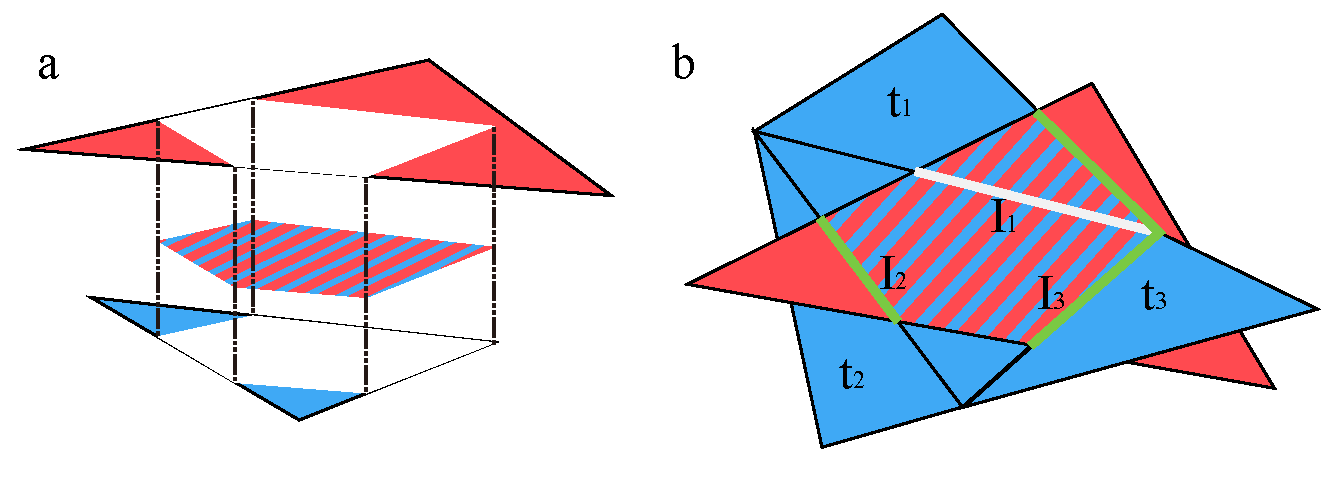
\includegraphics[width=3.5in]{coplanar}
\caption{a) Coplanar cases and the b) the possible configurations of the companion faces. In any configurations, their is no need to record the intersection of coplanar cases.}
\label{fig:coplanar}
\end{figure}

Consider two triangle faces $t_1$ and $t_2$ intersect within a common plane. Both $t_1$ and $t_2$ will divide each other into two areas---a convex overlapping area and exclusive parts (Fig. \ref{fig:coplanar}). Obviously, if we tessellate both $t_1$ and $t_2$ according to the boundary of overlapping area, we can guarantee that the tessellated meshes will not cross the boundary of any other meshes. In fact, many methods \cite{feito2013fast,zhou2016mesh} claim that tessellating faces according to this 2D-intersection result is necessary. However, in our method, we do not test whether $t_1$ and $t_2$ really intersect in 2D. We simply omit all coplanar situations, treating them as they do not intersect at all. This simplify our method, making it more robust and fast, while doing no harm to the topology correctness.

The key observation is that intersection in 2D does not create new valid edges. The word `valid` means the edge is necessary or possibly necessary for the final result mesh. We find that each intersection line segment in 2D is on the edges from input meshes. That means we can view 2D intersections as special cases of edge intersection. The only difference is that there can be up to three edge intersections in one 2D intersection (Fig. x). As we have discussed, edge intersection will be detected twice. That means we can rely on the companion triangle faces to detect intersections. There is more extreme case that the companion triangles are coplanar, meaning neither of them will record the intersection. However, in this case, the intersection is not valid. The two sides of the intersection are both retained or both dropped and we do not rely the it for tessellation.

\section{Deferred Tessellation}



\label{sec:tessellation}
After intersection computation, tessellation is performed on each intersecting triangle face and generate the intersection-free hybrid mesh. We call this stage as deferred tessellation because the tessellation happens until all valid intersections are computed. Ogayar-Anguita et. al. \cite{ogayar2015deferred} use Constrained Delaunay Triangulation (CDT) to perform deferred tessellation. They treat triangle faces as convex triangulation zones and intersections as constraints.

Our first try is to implement a robust CDT and apply to our method. However, we fail because of the dilemma of precision and efficiency. CDT algorithms \cite{chew1989constrained,preparata2012computational} usually require coordinates projection or intersection detection between arbitrary connections of vertices within triangulation zone. Because vertices may be implicitly represented in our method, these geometry predicates are hard to guarantee computation efficiency and precision simultaneously. Moreover, when there are more than two primitives, simply applying CDT omits the complexity of intersections between meshes. The intersections may intersect each other, introducing new vertices and splitting original intersection line segments (Fig. x). This breaks the assumption of most CDT algorithms and may lead to incorrect output topology.

To solve these problems, we first perform intersection refinement to eliminate any crossing or overlapping between intersections. After that, we perform conservative tessellation based on plane-based geometry, ensuring unconditional topology correctness. The word `conservative` means we tessellate face into polygons, not triangles. During tessellation, we organize intersections and generate an \emph{tess-graph}, which is a graph-like description of intersections. At last, we extract subfaces from tess-graph of each triangle face and construct the intersection-free hybrid meshes.

\subsection{Intersection Refinement}


The intersection vertices are not only introduced by intersection between an edge and a triangle, but also introduced by intersections of three triangles. It is not enough to find all of them by only triangle-triangle intersection tests. Also, because of degenerate cases, there will be other forms of intersections involving three or even more triangles. To make tessellation easier and more robust, we have to refine these intersections and all unusual conditions have to be removed before it.

Intersection refinement is performed in a local scope. For each intersecting face $t_i$, we collect all intersections on $t$ as a set $\bm{\Gamma}(t)=\{\mathbb{I}_{t}^i, i=0,1,2,...\}\cup\{\mathbb{I}_{t}^{e_i},i=0,1,2\}$ and refine them together. The set $\{\mathbb{I}_{t}^{e_i},i=0,1,2\}$ is the PBI-reps of the three edges of $t$. We treat edges as intersections for simplicity in this stage. The neighborhood component $\bm{\Psi}(\mathbb{I}_{t}^{e_i})$ is set as $\bm{0}$. Other components of $\mathbb{I}_{t}^{e_i}$ are straightforward to determine. Refinement on $\bm{\Gamma}(t)$ is done using only plane-based geometry predicates by the following three steps:

\vspace{0.5em}
\noindent \textbf{Collinear splitting}~~~~
Each intersection $\mathbb{I}_{t}^x$ are testing whether they are collinearly overlapping with other intersections. If yes, $\mathbb{I}_{t}^x$ is split by the end points of overlapping intersections (Fig. x). Because $\mathbb{I}_{t}^x$ may collinearly overlap more than one other intersection, the splitting may be deferred until all splitting points are found. The subroutine linear order of points (\S\ref{sec:substrates}) is used to sort these splitting points along $\mathbb{I}_{t}^x$. The PBI-reps of split segments inherit their father's except the second component the end points.

\vspace{0.5em}
\noindent \textbf{Coincidence elimination}~~~~
We merge coincidence intersections which have the same end points. Intersections are undirected so intersections with inverse end points are also coincident. The PBI-rep of the new intersection is inherited from either of the old one's except the neighborhood component $\bm{\Psi}$. We follow the merging rules below:
\begin{equation}
  \Psi_k(\mathbb{I}_{t}^{12})=\left\{
   \begin{array}{l}
   \Psi_k(\mathbb{I}_{t}^1)\mbox{ or }\Psi_k(\mathbb{I}_{t}^2),\ \mbox{ if } \Psi_k(\mathbb{I}_{t}^1)=\Psi_k(\mathbb{I}_{t}^2) \\
   \Psi_k(\mathbb{I}_{t}^1),\ \ \ \ \ \ \ \ \ \ \ \ \ \ \ \ \ \ \mbox{ if } \Psi_k(\mathbb{I}_{t}^2)=0  \\
   \Psi_k(\mathbb{I}_{t}^2),\ \ \ \ \ \ \ \ \ \ \ \ \ \ \ \ \ \ \mbox{ if } \Psi_k(\mathbb{I}_{t}^1)=0  \\
   \end{array}
  \right.
\end{equation}
, where $\mathbb{I}_{t}^1$ and $\mathbb{I}_{t}^2$ are old intersections and $\mathbb{I}_{t}^{12}$ is the new one.


\vspace{0.5em}
\noindent \textbf{Crossing intersection resolving}~~~~
After the process of two previous steps, there are no overlapping intersections in $\bm{\Gamma}(t)$. We check whether any pair of intersections intersect each other. The definition of \emph{intersect} does not include the situation that two intersections share end points. In Fig. x, we illustrate the only two situations. In both situations, one intersection is split by other, and the same splitting routine is used as in collinear splitting.

%\vspace{0.5em}
%There is one more thing that we give intersections generated (by merging or splitting) from the PBI-reps of edges  the positive directions. That means all intersections lies on triangle edges have a positive direction. Direction is defined by the direction of edge the intersection lies on.

\subsection{Tessellation by Tess-Graph}

So far, intersections are only independent data that store the coordinates and neighbouring information. To perform tessellation and extract subfaces, we need to organize them to reveal the topology. We use tess-graph for this purpose. A tess-graph is the graph description of the tessellated face topology. For each face to be tessellated, we construct a tess-graph according to the refined intersections. Nodes of tess-graph represent end points of intersections and undirectional connections between nodes represent intersections. The construction of tess-graph is straightforward and the reader will not have problem filling the details.

After we have tess-graph, we tessellate face and extract subfaces according to it. This is done by tracing loops on tess-graph. A valid loop that corresponds to a subface must satisfy two criterions: 1) the direction of loops should be coherent with the face normal, and 2) consecutive connections on the loop should be adjacent by circular order {\color{red}{Fig.?}}. After we find out all valid loops on tess-graph, the tessellation is done on that triangle face. More details are discussed in \S\ref{sec:}.

%In our implementation, we find that it is not easy to check whether the loop direction is coherent with face normal by plane-based geometry.

%First, We classify connections of tess-graph into two types: connections on face boundaries as \emph{boundary connections} and connections inside face as \emph{inner connections} by the whether they have positive directions. In the view of halfedge, inner connections represent two opposite halfedges but boundary connections represent only one. We add an attribute for each connection to identify their directions, and thus we get a directed version of Tess-graph. A sub-face is a halfedge loop on the directed Tess-graph. Extracting faces are process of searching for valid loops which meet certain geometry constraints. After all faces are extracted, all halfedges of directed Tess-graph should be used

%There two geometry constraints for valid loops. Second, consecutive connections on the loop should be adjacent by circular order {\color{red}{Fig.?}}. To meet these constraints, we sort the halfedges counter-clockwise for each nodes with more than two halfedges starting from them. This is implemented by using the divide-and-conquer framework of quick sort. During each recursion, we pick a random halfedge and split the rest into two sets according to the sign of two-line-on-plane comparison. To make the results of two-line-on-plane comparisons coherent, we assume that for each halfedge $h_i$, the normal directions of its plane-rep, denoted as $\vec{n}(h_i)$, meets the following criterion:
%\begin{equation}
%(\vec{n}(h_i) \times \vec{n}_0) \cdot \vec{l}(h_i) > 0,
%\end{equation}
%where $\vec{n}_0$ is the normal of the face, and $\vec{l}(h_i)$ is the direction of $h_i$. The plane-rep of halfedge can be inherited from the corresponding connections from the undirected Tess-graph. Since we {\color{red}{guarantee that each connection has a plane-rep //need insert//}}, sorting can be exactly and fast performed. After connections are sorted in each nodes, we can know which connections are adjacent and what is the right direction during the loop search.


\section{Face Classification, p->e->f, patial sort}

\label{sec:classification}
This stage traverses all candidate faces in the Linked Halfedge, and classifies which of them belong to the final mesh. Classification is done by evaluating the indicator vector of each face {\color{red}{(indicator vector?)}}. During this process, we take advantage of P-rep to ensure unconditional correct classification. In addition, since we maintain the intra-primitive geometry connectivity and inter-primitive geometry connectivity in Linked Halfedge, we can utilize the space coherence of face indicator vectors to accelerate this process.

In this section, we will first give an overall framework of face classification, and then introduce how to classify each individual face. At last, we discuss how to accelerate this process by caching intermediate results.

\subsection{Framework}

The space coherence of indicator vectors means neighboring faces could share the same indicator vector, or most components of indicator vectors. For example, given two neighboring faces $t_1$ and $t_2$, indicator vectors $\boldsymbol{\Lambda}(t_1)$ and $\boldsymbol{\Lambda}(t_2)$ would often be the same. Only when there is boundary of some meshes, say $P_k$, on the shared edge $e(t_1, t_2)$ and split $t_1$ and $t_2$ in two sides, the corresponding components $\boldsymbol{\Lambda}(t_1, P_k)$ and $\boldsymbol{\Lambda}(t_2, P_k)$ can be different. And other components of $\boldsymbol{\Lambda}(t_1)$ and $\boldsymbol{\Lambda}(t_2)$ will remain the same. If we can compute the indicator changes between neighboring faces efficiently, we can start from a single face with a indicator vector as the seed, propagating to all faces with geometry connectivity, reusing indicator vectors according to the spatial coherence and classifying faces very fast.


Fortunately, in the Linked Halfedge, it is straightforward to know whether $\boldsymbol{\Lambda}(t_1, P_k)$ and $\boldsymbol{\Lambda}(t_2, P_k)$ are different, because it means $e(t_1, t_2)$ will be on the boundary of $P_k$, and there will be corresponding I-reps stored on $e(t_1, t_2)$. In addition, both $\boldsymbol{\Lambda}(t_1, P_k)$ and $\boldsymbol{\Lambda}(t_2, P_k)$ can be computed efficiently according to the I-reps (details in Section \ref{sec:individual}). We outline our classification method in Algorithm 1.

\begin{algorithm}
\caption{Fast Face Classification}
\label{code:floodfill}
\textbf{Input: } Linked Halfedge structure $\Omega$

\textbf{Output: } Classification of each face $f(\boldsymbol{\Lambda}(t_i)), t_i \in \Omega$


\begin{algorithmic}[1]
\State Select a proper seed face $t_s$
\State Compute the first indicator vector $\boldsymbol{\Lambda}(t_s)$
\State \Call{propagate} { $t_s$ , $\boldsymbol{\Lambda}(t_s)$}
\State
\Function{propagate}{ $t_c$ , $\boldsymbol{\Lambda}(t_c)$}
    \State Compute $f(\boldsymbol{\Lambda}(t_c))$
    \For {each neighboring face $t_i^c$}
        \If {there are I-reps $\{{\mathbb{I}}_k\}$ on $e(t_i^c, t_c)$}
            \State $\boldsymbol{\Lambda}(t_c), \{{\mathbb{I}}_k\} \Longrightarrow \boldsymbol{\Lambda}(t_i^c)$
            \State \Call{propagate} { $t_i^c$ , $\boldsymbol{\Lambda}(t_i^c)$}
        \Else
            \State \Call{propagate} { $t_i^c$ , $\boldsymbol{\Lambda}(t_c)$}
        \EndIf
    \EndFor
\EndFunction
\end{algorithmic}
\end{algorithm}

\subsection{Precise Seed Generation}

Our classification method starts from computing the seed indicator vector using point-in-polyhedron test \cite{ogayar2005point}. Conventionally, the barycenter of the face is used for the test to compute the indicator vector of the whole face. This is because the whole face is classified as a whole, and every inner point will have the same indicator vector. However, the coordinates of the inner points cannot be exactly represented by float point numbers, which may lead to wrong predicates, especially when it is an on-boundary case. Therefore, we use the original vertices, whose exact coordinates are known, for point-in-polyhedron test. For this reason, only tessellated faces with at least one original vertex can be the seed face. The point-in-polyhedron test is guaranteed to be exact. On the other hand, efficiency is not so important as there will not be many such tests. If ray-trace algorithms (e.g., \cite{frisken2002simple}) are used, the octree constructed during space division can be used for acceleration \cite{havran1999summary}.

However, using point on the boundary instead of an inner one has another problem. Given a face $s$ (may not be triangle) and one of its vertex $v_b^i(s)$, the vertex indicator $\boldsymbol{\Lambda}(v_{i}(s), P_k)$ may cause ambiguity to deduce the face indicator $\boldsymbol{\Lambda}(s, P_k)$. In {\color{red}{Fig. ?}}, $\boldsymbol{\Lambda}(v_b^1(s), P_k) = on$, then $\boldsymbol{\Lambda}(s, P_k)$ can be any of the four conditions. We solve this problem by trying other vertices in $s$ for ambiguous indicators. If all vertices indicators are $on$ and the ambiguity cannot be resolved, the current face is not proper for being the seed and we select a new one instead.

\subsection{Fast and Exact Classification}

\label{sec:individual}

Feito et. al. \cite{feito2013fast} had noticed that intersection neighborhood can be used for fast classification of faces around that intersection. According to their method, faces adjacent to intersection have neighbors from other primitive(s) that define the position and orientation for each other, by which the indicators are determined. However, Feito et. al. did not give detail description of how to implement an exact and robust classification. Their implementation of using vertex coordinates might misclassify faces by numeric errors and fail in degenerate cases. Because geometry connectivity is used, local misclassification can be spread to the neighborhoods, leading to errors in wide ranges.

We develop an classification method that is unconditionally robust and exact based on the idea of using intersection neighborhood information. The neighborhood information is stored in the context component of I-reps during previous stages . In the following, we discuss the conditions that the face to be classified is a triangle. If the face is not a triangle, we select a triangle slice of the face instead, as the whole face is guaranteed to be classified together. Note that the chosen slice should contain the edge where the I-reps lie, by which we compute the new indicators.

Given a face $t_i$ to be classified and an I-rep $\boldsymbol\Gamma$ of intersection on one of $t_i$'s edge, we denote the three corners it as $v_{b*}^{0}(t_i), v_{b*}^{1}(t_i), v_b^2(t_i),$ where the subscript $*$ means the vertices are on the edge where $\boldsymbol\Gamma$ lies. We also denote the context component of $\boldsymbol\Gamma$ as $C_{P_h \backslash P_j}$, meaning $t_i$ is from primitive $P_j$ and intersects primitive $P_h$. From previous discussion (section \ref{sec:ir}){\color{red}{may be more than one}}, we know there are two types of intersection context---face neighborhood and edge neighborhood. In both conditions, the one or two faces involving in the context split the space into two in and out space by its (their) orientation(s). We will see that under such division (denoted as $\boldsymbol{D}(C_{P_h \backslash P_j})$), we can compute $\lambda(t_i, P_j)$ exactly.

Since the faces involving in $C_{P_h \backslash P_j}$ is part of primitive $P_j$, the space division $\boldsymbol{D}(C_{P_h \backslash P_j})$ is homogeneous with the space division by $P_j$ in neighborhood of $\mathbb{I}$. The basic idea is to choose one point $v_x(t_i)$ on $t_i$ close enough to $\mathbb{I}$ to compute $\lambda(v_x(t_i), P_j)$, and then compute $\lambda(t_i, P_j)$ accordingly. However, the problem is that we cannot find such a $v_x(t_i)$ that can be represented exactly, which means robust classification cannot be performed. Fortunately, we observe that we can choose $v_b^2(t_i)$, which is not so close to $\mathbb{I}$ instead. To illustrate, assume there is another point $v_{x'}(t_i)$ inside of $t_i$ that is very close to $v_b^2(t_i)$ ({\color{red}{Fig. x}}). Because all inner points of $t_i$ have the same indicator, $\lambda(v_x(t_i), P_j) = \lambda(v_{x'}(t_i), P_j)$. On the other hand, we find that $\lambda(v_{x'}(t_i), P_j)$ and $\lambda(v_b^2(t_i), P_j)$ are always equal under division $\boldsymbol{D}(C_{P_h \backslash P_j})$ ({\color{red}{see Appendix \ref{app:profind}}}). Therefore, $\lambda(v_b^2(t_i), P_j)$ is equal to $\lambda(v_x(t_i), P_j)$ under $\boldsymbol{D}(C_{P_h \backslash P_j})$, and are coherent with $\lambda(t_i, P_j)$ under the division of whole primitive $P_j$. One additional thing is that when $\lambda(v_2(t_i), P_j)=on$, then $\lambda(t_i, P_j)$ can be either $same$ or $oppo$. The normal orientation test have to be performed to eliminate such ambiguity.



\section{Implementation}

\vspace{0.5em}
\textbf{Seed Indicator Vector Generation.} Our method of generating the first indicator vector will fail on extreme conditions when all faces in Linked halfedge are coincident with more than one primitive face (e.g., the union of the same mesh). In order to be robust, we use the high-precision face barycenter with the point-in-polyhedron test to generate the seed indicator vector instead after several failures of choosing a proper seed face.

\vspace{0.5em}
\noindent \textbf{Exact Face Classification.} In Linked halfedge, all the supporting planes of faces and all the vertices can be exactly represented. Based on that, when computing the new indicator according to I-reps, we can use BSP techniques similar to \cite{bernstein2009fast} to conduct robust predicates. Since the intersection context is neither face or edge, the space division planes in each BSP will be no more than two, which guarantees fast construction and classification.


\vspace{0.5em}
\noindent \textbf{Continuous operations.}


\vspace{0.5em}
\noindent \textbf{Parallel.}


\vspace{0.5em}
\noindent \textbf{Lazy intersection.}



\vspace{0.5em}
\noindent \textbf{Caching Evaluation Results}
If the CSG tree is large, with hundreds of primitive nodes, computing $\lambda_f(x)$ from $\boldsymbol{\Lambda}(x)$ for every face can be costly. Thanks to the space coherence of $\boldsymbol{\Lambda}(x)$, we can save the computation time by caching the evaluation result of Boolean operations.

The basic cache strategy is to cache final result, that is, the value of $\lambda_f(x)$. We know indicator vector $\boldsymbol{\Lambda}$ will not change if there is no intersections during spreading. That means the final classification $\lambda_f(x)$ will not change, too. Thus, those faces sharing the same $\boldsymbol{\Lambda}$ can be classified as a whole.

Also, we can perform intermediate results cache. We noticed that the Boolean expression can be simplified if some components of $\boldsymbol{\Lambda}(x)$ is fixed. For example, assume we have a Boolean expression $P_1\cup (P_2\cap P_3-P_4)$. Given the values of two indicators $\lambda_1(x)=out$, $\lambda_2(x)=in$, the expression can be rewritten as $out\cup (in\cap P_3-P_4)$. Using the combination rules we can simplify the expression as $P_3-P_4$. This fact is important because for a large CSG, a certain primitive, denoted as $P_x$, often only intersects with a few other primitives, like, $\Theta(P_x)= \{P_{n_1}, P_{n_2}, \cdots, P_{n_k}\}$. That means all the faces in $P_x$ has the same indicators for the primitives not in $\Theta(P_x)$. Therefore, we can first determine these fixed indicators and simplify the Boolean function, and then use simplified one to compute the final indicator for each faces in $P_x$.

\vspace{0.5em}
\noindent \textbf{Proof of Indicator Equality}
\label{app:profind}

Using the notation in section \ref{sec:individual}, we prove the equality of $\lambda(v_{x'}(t_i), P_j)$ and $ \lambda(v_b^2(t_i), P_j)$ under the space division $\boldsymbol{D}(C_{P_h \backslash P_j})$.

Given $v_{x'}(t_i)$ can be arbitrarily close to $v_b^2(t_i)$, if $\lambda(v_b^2(t_i), P_j) = in | out$, the equality holds because of the continuity of space. If $\lambda(v_b^2(t_i), P_j) = on$, we divide the proof of equality into two parts according to the type of intersection context. If $C_{P_h \backslash P_j}$ is face neighboring type, $\boldsymbol{D}(C_{P_h \backslash P_j})$ is a single face, say, $t_0^c$. We have already know that the other two corners $v_{b*}^{0}(t_i)$ and $v_{b*}^{1}(t_i)$ are on $s_0$. Since $\lambda(v_b^2(t_i), P_j) = on$, we know $v_b^2(t_i)$ is on $t_0^c$, too. There comes the conclusion that the whole triangle $t_i$ is coplanar with $t_0^c$. Therefore, $v_{x'}(t_i)$ is on $t_0^c$ and $\lambda(v_{x'}(t_i), P_j) = on$, too. On the other hand, if $C_{P_h \backslash P_j}$ is edge neighboring type, $\boldsymbol{D}(C_{P_h \backslash P_j})$ are two neighboring faces (denoted as $t_1^c, t_2^c$). We know that both $v_{b*}^{0}(t_i)$ and $v_{b*}^{1}(t_i)$ are on the shared edge $e(v_{b*}^{0}(t_i), v_{b*}^{1}(t_i))$. It means both vertices are on both $t_1^c$ and $t_2^c$. Using the same deduction of the first condition, we can conclude $\lambda(v_{x'}(t_i), P_j) = on$ whenever $\lambda(v_b^2(t_i), P_j) = on$.

\section{Experiments}

\section{Summary}

In this paper, we proposed a novel method to evaluate CSG with triangular mesh primitives. It is able to efficiently perform non-incremental evaluation of large CSG with massive faces. The key idea of our approach is to use the local coherence of face space labels to accelerate face membership classification. A two-level grouping framework is developed to group neighboring faces together and thus space labels can be shared within each group. This scheme saves much time for space label computation, which is often very time-consuming for conventional Boolean evaluation algorithms. Additionally, in order to be robust, plane-based geometry computation is introduced into the intersection computation step of our approach. Experiments have verified the proposed approach is more efficient than the state-of-the-art techniques while retaining robustness and stability. We will further investigate the robust tessellation in future.



\appendices


%\newpage
\bibliographystyle{IEEEtran}
\bibliography{IEEEabrv,citation}


%\newpage

\begin{IEEEbiography}[{\includegraphics[width=1in,height=1.25in,clip,keepaspectratio]{rui}}]{Rui Wang}
is currently a postgraduate student at the Department of Computer Science and Technology, the Shanghai Jiao Tong University. His main research interests include real-time computer graphics and virtual reality applications.
\end{IEEEbiography}

% if you will not have a photo at all:
\begin{IEEEbiography}[{\includegraphics[width=1in,height=1.25in,clip,keepaspectratio]{xudong}}]{Xudong Jiang}
received his Master degree in Computer Science from Shanghai Jiao Tong University in 2014. He is currently working in Autodesk China Research \& Development Center. His research interest includes computer-aided geometric design and solid modeling.
\end{IEEEbiography}


\begin{IEEEbiography}[{\includegraphics[width=1in,height=1.25in,clip,keepaspectratio]{hongbo}}]{Hongbu Fu}
is an Associate Professor in the School of Creative Media, City University of Hong Kong. He received the PhD degree in computer science from the Hong Kong University of Science and Technology in 2007 and the BS degree in information sciences from Peking University, China, in 2002. His primary research interests fall in the fields of computer graphics and human computer interaction. He has served as an associate editor of The Visual Computer, Computers \& Graphics, and Computer Graphics Forum.
\end{IEEEbiography}


\begin{IEEEbiography}[{\includegraphics[width=1in,height=1.25in,clip,keepaspectratio]{sheng}}]{Bin Sheng}
received his BS degree in computer science from Huazhong University of Science and Technology in 2004, MS degree in software engineering from University of Macau in 2007, and PhD Degree in computer science from The Chinese University of Hong Kong in 2011. He is currently an associate professor in the Department of Computer Science and Engineering at Shanghai Jiao Tong University. His research interests include virtual reality, computer graphics, and image-based techniques.
\end{IEEEbiography}

\begin{IEEEbiography}[{\includegraphics[width=1in,height=1.25in,clip,keepaspectratio]{wu}}]{Enhua Wu}
received the BS degree from Tsinghua University in 1970, and the PhD degree from the University of Manchester (UK) in 1984. He is currently a research professor at the Institute of Software, Chinese Academy of Sciences, and Fellow of China Computer Federation. He has also been teaching at the University of Macau since 1997, where he is currently an Emeritus Professor. His research interests include realistic image synthesis, virtual reality, and scientific visualization. He has served as an associate editor of The Visual Computer, Computer Animation and Virtual Worlds.
\end{IEEEbiography}





\end{document}


